\documentclass[11pt]{article}
\usepackage[margin=1in]{geometry}
\usepackage{amsmath,amssymb,amsthm,bm}
\usepackage{booktabs,multirow,array,tabularx}
\usepackage{graphicx,xcolor,microtype}
\usepackage[font=small,labelfont=bf,labelsep=colon]{caption}
\usepackage{subcaption}
\usepackage[ruled,vlined,linesnumbered]{algorithm2e}
\usepackage[numbers,sort&compress]{natbib}
\usepackage[hidelinks]{hyperref}
\usepackage{enumitem}
\usepackage[section]{placeins}
\setlist{nosep}
\emergencystretch=3em
\renewcommand{\figurename}{Fig.}
\newtheorem{theorem}{Theorem}[section]
\newtheorem{lemma}[theorem]{Lemma}
\newtheorem{proposition}[theorem]{Proposition}
\newtheorem{corollary}[theorem]{Corollary}
\theoremstyle{definition}
\newtheorem{assumption}[theorem]{Assumption}
\newtheorem{definition}[theorem]{Definition}
\newtheorem{remark}[theorem]{Remark}
\newcommand{\R}{\mathbb{R}}
\newcommand{\norm}[1]{\left\lVert #1 \right\rVert}
\newcommand{\Kt}{\tilde K}
\newcommand{\Kh}{\hat K}
\newcommand{\kh}{\hat\kappa}
\newcommand{\eps}{\varepsilon}
\newcommand{\Ghat}{\hat G}
\newcommand{\T}{^{\mathsf T}}
\newcommand{\bigO}{\mathcal{O}}
\newcommand{\nnz}{\operatorname{nnz}}
\newcommand{\dsus}{\textunderscore\penalty5000\hskip0pt\relax}
\newcommand{\ds}[1]{{\ttfamily\let\_\dsus#1}}
\newcommand{\lead}[1]{\emph{#1}\ }
\graphicspath{{fig/}}
\makeatletter\newcommand{\inputrows}[1]{\@@input #1 }\makeatother
\newcommand{\cZero}{1.10}
\newcommand{\directSamples}{$3.9\times10^{17}$}
\newcommand{\refinedSamples}{$7.3\times10^{3}$}


\title{Certified Classical and Quantum Linear Solves inside a Production Interior-Point Method:\\ Equilibration, Low-Precision Refinement, and Conditions for a Quantum Advantage}
\author{Authors\thanks{Author names and affiliations to be inserted. Correspondence: \texttt{ldrresearch2025@gmail.com}.}}
\date{October 2026}

\begin{document}
\maketitle

\begin{abstract}
Every iteration of a primal--dual interior-point method (IPM) solves a symmetric indefinite Karush--Kuhn--Tucker (KKT) system whose conditioning deteriorates as the barrier parameter vanishes. We develop a certified inexact-solve framework for the KKT callback of the production solver \textsc{cvxopt}, in which classical Krylov and simulated quantum linear solvers are subject to one acceptance test, one fallback protocol and one strict accounting, and we combine it with four methodological components: per-iteration symmetric equilibration of the augmented KKT matrix, a combined block-forcing and backward-error test, a latency-optimised GPU MINRES kernel, and a quantum solver that runs a minimax-optimal inversion polynomial at fixed low precision inside classical iterative refinement, optionally on a positive definite null-space target. We prove that the refined quantum solver contracts the residual by $\xi\le\eps+(1+\eps)\kh\zeta$ per round, bound its block-encoding queries, and show that its circuit depth is independent of the final accuracy, that equilibration shortens it by at least $\kappa(\Kt)/\kh$, and that an advantage over MINRES per Newton direction requires dense, well-equilibrated systems and is bounded by the ratio $k/R$ of Krylov iterations to refinement rounds. Empirically, equilibration lowers the KKT condition number by a median $4.3\times10^{4}$ on \ds{sparse\_banded} and makes unpreconditioned MINRES fallback-free on every synthetic run up to dimension $79\,360$ and up to $9.4\times$ faster than sparse LDL$\T$ under high fill-in, whereas the factorisation remains fastest on 40 of 48 Maros--M\'esz\'aros QPs. In simulation, the quantum components reduce block-encoding queries per solve by $237\times$, circuit depth by $2.70\times$ (a further $4.0\times$ on the null-space target) and samples per solve from \directSamples{} to \refinedSamples{}, and the IPM converges on quantum-produced directions alone on 8/8 instances with ideal readout and on 39/40 seeded finite-sampling runs. All quantum results are classical simulations of ideal circuits; no end-to-end quantum speed-up is demonstrated.
\end{abstract}

\noindent\textbf{Keywords:} interior-point methods; KKT systems; inexact Newton directions; equilibration; Krylov methods; GPU computing; quantum linear-system algorithms; iterative refinement; block encoding.

\section{Introduction}\label{sec:intro}
Interior-point methods solve convex quadratic programs (QPs) in a few dozen Newton iterations, and each iteration requires the solution of a KKT linear system. Production solvers factorise this system---by a sparse LDL$\T$ decomposition of the augmented matrix or a Cholesky decomposition of a reduced one---and the factorisation dominates the run time whenever its fill-in is severe. Replacing it by an iterative Krylov method is a classical idea~\cite{gondzio2012matrixfree,bergamaschi2004preconditioning}, and the convergence theory of inexact IPMs prescribes how accurate each direction must be~\cite{bellavia1998inexact,aljeiroudi2009convergence,gondzio2013convergence,dexter2022inexact}. The same step has more recently been proposed as the point of insertion for quantum linear-system algorithms inside quantum IPMs~\cite{kerenidis2020qipm,augustino2023qipm,wu2023inexact,mohammadisiahroudi2024efficient,mohammadisiahroudi2025improvements}, whose end-to-end practicality has been questioned by resource analyses~\cite{dalzell2023endtoend}.

Whether an inexact or a quantum KKT solver is useful inside an IPM depends on three questions: how accurate a Newton direction must be for the outer iteration to converge; how that accuracy can be certified at a cost below that of the solve itself; and which solvers can deliver it on the matrices that an IPM actually produces. Existing studies address these questions separately. Inexact-IPM analyses fix the forcing condition but are typically evaluated with purpose-built IPMs and preconditioners; quantum-IPM demonstrations simulate phase-estimation HHL on linear systems of dimension at most 16 and reach a precision of about $10^{-4}$~\cite{mohammadisiahroudi2025improvements}; and complexity bounds for quantum IPMs are stated in terms of a condition number that grows without bound along the central path. No study has subjected classical and quantum solvers to the same certification inside an unmodified production IPM, and none has quantified which methodological choices reduce the resources a quantum solver needs, by how much, and how far the reduced cost remains from a quantum advantage.

This paper addresses these questions within a single framework. We use the \texttt{kktsolver} callback of \textsc{cvxopt} \texttt{coneqp}~\cite{cvxopt,andersen2011ipm}, which allows any solver to replace the KKT factorisation while the rest of the algorithm---Nesterov--Todd scaling, the predictor--corrector scheme, step lengths and stopping tests---remains untouched. Every solver, classical or quantum, is subject to the same acceptance test, the same classical-fallback protocol and the same accounting, so that a reported success means that the IPM converged on directions produced by the solver under test alone. Fig.~\ref{fig:summary} summarises the principal outcomes.

\begin{figure}[t]\centering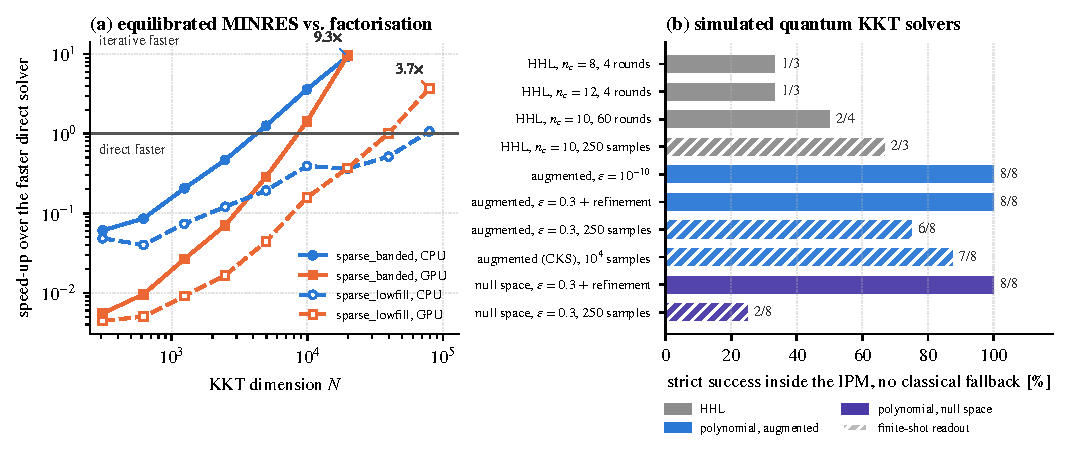
\includegraphics[width=\textwidth]{fig_summary.pdf}
\caption{Principal outcomes. (a) Speed-up of equilibrated MINRES over the faster of the two direct solvers (ratio of median whole-run times) versus KKT dimension, on \ds{sparse\_banded} (high Cholesky fill-in, solid) and on the control family \ds{sparse\_lowfill} (low fill-in, dashed), on the CPU and on a Tesla T4 GPU. (b) Share of IPM runs in which a simulated quantum KKT solver drove the unmodified solver to the optimum with every direction accepted and no classical fallback.}\label{fig:summary}
\end{figure}

\paragraph{Methodological contributions.} The contributions are the following.
\begin{enumerate}[leftmargin=2.2em,label=\textbf{C\arabic*.}]
\item \emph{A certified inexact-solve framework for a production IPM} (Section~\ref{sec:method}). A combined acceptance test---per-block forcing $\eta=0.1$ together with a normwise backward error $\omega\le10^{-9}$---certifies every direction at 22--34\,\% more Krylov work than the cheapest single test that is also fallback-free, and a three-level accounting (accepted, fallback-free, strict) separates the contribution of the solver under test from that of the safeguards. The framework applies unchanged to classical Krylov methods, noisy exact solves, HHL and polynomial quantum solvers.
\item \emph{Per-iteration symmetric equilibration of the augmented KKT matrix} (Sections~\ref{sec:equil} and~\ref{sec:criteria}). Ruiz equilibration applied to every new KKT matrix, rather than once to the problem data, lowers the condition number by a median $4.3\times10^{4}$ on \ds{sparse\_banded} and $5.4\times10^{3}$ on \ds{dense\_kappa}. It makes unpreconditioned MINRES fallback-free on all synthetic runs, whereas every unscaled variant needs fallback in 38--50\,\% of them. For the quantum solver, Corollary~\ref{cor:equil} shows that the same transformation shortens the circuit by at least the factor by which it reduces the condition number ($1.2\times10^{5}$ and $1.2\times10^{4}$ at $\eps=0.3$).
\item \emph{A measured precision law for Newton directions} (Section~\ref{sec:noise}). At every IPM tolerance $\tau$ from $10^{-8}$ to $10^{-4}$, the largest relative direction error tolerated on every instance lies between $\tau/10$ and $\tau$. This fixes the accuracy target of any inexact or quantum solver and, combined with Corollary~\ref{cor:precision}, implies that refinement needs only $\bigO(\log(1/\tau))$ rounds.
\item \emph{A latency-optimised GPU MINRES kernel and a controlled scaling study} (Sections~\ref{sec:gpumodel}, \ref{sec:scaling} and~\ref{sec:gpu}). A kernel with one host synchronisation per iteration, fused vector updates and adaptively spaced convergence checks is $1.14$--$1.29\times$ faster per iteration than a direct CuPy transcription. Equilibrated MINRES overtakes the sparse LDL$\T$ factorisation at $N\approx5\times10^{3}$ under high fill-in and is $9.4\times$ faster at $N=19\,840$; the GPU pays off from $N\approx2\times10^{4}$ ($3.75\times$ at $79\,360$). A low-fill control family and 48 Maros--M\'esz\'aros QPs delimit the regime in which these gains hold.
\item \emph{A low-precision refined polynomial quantum solver} (Sections~\ref{sec:qpolysolver}--\ref{sec:refine} and~\ref{sec:qpoly}--\ref{sec:qshots}). The minimax-optimal inversion polynomial of S\"underhauf et al.~\cite{sunderhauf2025polynomials}, executed at fixed precision $\eps=0.3$ inside classical iterative refinement with a few hundred samples per round, needs $2.70\times$ fewer walk steps than the Childs--Kothari--Somma expansion and $237\times$ fewer block-encoding queries per solve than a high-precision circuit. It drives the unmodified IPM to the optimum with every direction quantum-produced on 8/8 instances with ideal readout and on 39/40 seeded runs at $4\,000$ samples per round. We identify the mechanism of the remaining failures: directions accepted close to the forcing threshold lengthen the IPM run into regions of larger condition number.
\item \emph{A positive definite null-space target with a closed-form polynomial} (Sections~\ref{sec:qspd} and~\ref{sec:oss}). The orthogonal-subspace system of inexact-feasible quantum IPMs is positive definite, so a shifted Chebyshev polynomial with closed-form coefficients and degree $\bigO(\sqrt{\kappa}\log(\kappa/\eps))$ suffices. Inside the IPM it needs $4.0\times$ fewer walk steps than the augmented target; Corollary~\ref{cor:oss} gives the criterion under which it is the cheaper target and explains why its advantage vanishes late in the run.
\item \emph{A complexity analysis with explicit conditions for a quantum advantage} (Section~\ref{sec:theory}). Theorem~\ref{thm:refine} bounds the contraction, the number of rounds and the block-encoding queries of the refined solver; three corollaries quantify the effect of precision, equilibration and the choice of target; and Proposition~\ref{prop:cost} states when the hybrid scheme can be cheaper than classical MINRES per Newton direction. The analysis shows that an advantage is possible only for dense, well-equilibrated systems, that it is polynomial and bounded by the ratio $k/R$ of Krylov iterations to refinement rounds, and it locates our measurements relative to that boundary (Fig.~\ref{fig:qresources}).
\end{enumerate}

\paragraph{Significance.} On the classical side, the results show that equilibration alone, without a preconditioner, makes a Krylov solver a certified and competitive replacement for the factorisation whenever fill-in is the bottleneck and the problem is regular, and that latency rather than arithmetic decides where a GPU kernel pays off. On the quantum side, the three dominant cost drivers of a QLSA inside an IPM---the condition number, the required precision and the readout of a classical vector---can each be reduced by orders of magnitude through classical pre- and post-processing that is cheap relative to the solve: equilibration acts on the condition number, low-precision refinement removes the $1/\eps_f^{2}$ sample dependence of direct readout and decouples the circuit depth from the IPM tolerance, and the choice of polynomial and target lowers the constants. These reductions apply to any QLSA-based IPM, and Proposition~\ref{prop:cost} quantifies the gap that remains. All quantum results are classical simulations of ideal circuits with oracle access to the block encoding and state preparation; they establish algorithmic feasibility and relative resource requirements, not a speed-up over classical solvers, and at the simulated sizes the absolute query counts exceed the classical cost by many orders of magnitude.

\paragraph{Organisation.} Section~\ref{sec:related} reviews the related literature. Section~\ref{sec:setting} introduces the KKT system of \texttt{coneqp} and its conditioning. Section~\ref{sec:method} presents the methodology: the certified solve protocol, equilibration, the MINRES kernel and the quantum solvers. Section~\ref{sec:theory} contains the complexity analysis. Section~\ref{sec:setup} describes the experimental setup, and Sections~\ref{sec:classical} and~\ref{sec:quantum} report the classical and quantum results. Section~\ref{sec:discussion} discusses significance, the outlook for a quantum advantage and the limitations, and Section~\ref{sec:conclusion} concludes. The appendices document reproducibility, the SDPLIB results and the replication across six computing sessions.

\section{Related work}\label{sec:related}
\subsection{Inexact interior-point methods and the conditioning of KKT systems}
Bellavia~\cite{bellavia1998inexact}, Al-Jeiroudi and Gondzio~\cite{aljeiroudi2009convergence} and Gondzio~\cite{gondzio2013convergence} establish forcing conditions of the form $\norm{r}\le\eta\mu$ under which an inexact IPM converges; Gondzio's analysis for convex QP requires the residual bound only in the complementarity block, which is related to our per-block test. Zanetti and Gondzio~\cite{zanetti2023stopping} derive IPM-specific termination criteria for CG and MINRES that estimate the IPM indicators inside the Krylov loop; they require access to the current iterate, which the \texttt{kktsolver} interface of \texttt{coneqp} does not provide, but our measurement of over-solving (Section~\ref{sec:spectrum}) quantifies what such a criterion could save. The boundedness of the unreduced (or suitably scaled) KKT matrix as $\mu\to0$ under strict complementarity and linear independence, in contrast to the $\bigO(\mu^{-2})$ growth of reduced and normal-equation systems, is established in~\cite{greif2014bounds,morini2016spectral}, and the benign structure of the ill-conditioning in~\cite{wright1998illconditioning,forsgren1996conditioning}; the general saddle-point background is surveyed in~\cite{benzi2005saddle}. In this terminology, the KKT matrix of \textsc{cvxopt} with its $-I$ block is the augmented form, and our contribution is the measured condition-number trajectory after symmetric equilibration and its consequences for classical and quantum solvers. Preconditioners for IPM sequences~\cite{bergamaschi2004preconditioning,gondzio2022generalpurpose,bellavia2015updating,pougkakiotis2021ippmm} and randomised Nystr\"om preconditioning~\cite{frangella2023nystrom,chu2026nystrom} are complementary; Section~\ref{sec:notadopted} shows that the low-rank premise of the latter does not hold on our families.

\subsection{Scaling, preconditioning and Krylov kernels on GPUs}
Ruiz equilibration~\cite{ruiz2001scaling,knight2014symmetry} is applied by OSQP~\cite{stellato2020osqp} once to the problem data; we apply it to the barrier KKT matrix at every IPM iteration. That Krylov methods on GPUs are bounded by synchronisation latency is known from the pipelined-CG literature~\cite{ghysels2014pipelined}; recent GPU IPM solvers~\cite{chen2025cuclarabel,pacaud2026condensed,regev2023hykkt} prefer direct factorisation on the device, and first-order GPU solvers~\cite{schubiger2020gpu,lu2025cupdlp} avoid the KKT solve altogether. Mixed-precision iterative refinement~\cite{carson2018three,wilkinson1963rounding} motivates our test of single-precision inner solves. For benchmarking we follow the performance-profile methodology of Dolan and Mor\'e~\cite{dolan2002benchmarking} and use the Maros--M\'esz\'aros collection~\cite{maros1999repository}, the standard real-world test set for convex QP solvers~\cite{stellato2020osqp}. Recycled Krylov methods for sequences of systems~\cite{parks2006gcrodr,wang2007rminres} and learned deflation spaces~\cite{luo2024neurkitt} address the growth of the iteration count that we measure in Section~\ref{sec:spectrum}; learned surrogates of the IPM linear solve~\cite{gao2024ipmlstm} reach residuals of about $10^{-2}$ and serve as warm starts rather than replacements.

\subsection{Quantum linear-system algorithms in optimisation}
HHL~\cite{harrow2009quantum}, its polynomial successors based on linear combinations of unitaries and quantum signal processing~\cite{childs2017quantum,gilyen2019qsvt,martyn2021grand,lin2020filtering,tong2021fastinversion}, and solvers with optimal $\bigO(\kappa\log(1/\eps))$ query complexity~\cite{costa2022optimal,dalzell2024shortcut} provide the quantum linear-algebra primitives; block-encoding constructions are surveyed in~\cite{camps2024blockencoding,gribling2024lcu}, and the textbook treatment of quantum optimisation in~\cite{nannicini2025book}. Aaronson's caveats~\cite{aaronson2015fineprint} and the tomography lower bounds of van Apeldoorn et al.~\cite{vanapeldoorn2023tomography} explain why extracting a classical solution costs at least $\Omega(N/\eps)$ state preparations, and dequantisation results~\cite{tang2019dequantize} delimit the regime in which low-rank structure removes any advantage. Quantum IPMs~\cite{kerenidis2020qipm,augustino2023qipm,wu2023inexact,mohammadisiahroudi2024efficient,mohammadisiahroudi2025improvements} use iterative refinement to escape the $1/\eps$ dependence of tomography; the standalone analysis of that scheme, with simulator and hardware experiments on systems of dimension 8 and 64, is due to Harkness et al.~\cite{harkness2026ir}, and the resource estimate for an end-to-end quantum IPM to Dalzell et al.~\cite{dalzell2023endtoend}. Inexact-feasible quantum IPMs~\cite{augustino2023qipm,wu2023inexact} solve the Newton system in a basis of the null space of the equality constraints (the orthogonal-subspace system), which preserves primal feasibility under inexact solves and yields a positive definite target. The VQE-based cutting-plane study of Ozbaygin, Kocuk and Moran~\cite{ozbaygin2026vqe} for SDP identifies power-of-two padding, Pauli density and tomography as practical obstacles to a variational separation oracle, all three of which we quantify for KKT matrices.

\subsection{Positioning}
The present study differs from the quantum-IPM demonstrations above in four respects: the IPM is an unmodified production solver rather than a purpose-built one; every quantum direction is subject to the same acceptance test and strict accounting as the classical ones, so that a success means that the IPM converged on quantum directions alone; the quantum solver is a walk-level polynomial solver operated at low precision inside refinement rather than phase-estimation HHL; and the resource reductions of each methodological component are both measured and derived in closed form, together with the conditions under which they could amount to an advantage. It differs from the inexact-IPM literature in that the classical Krylov results rest on equilibration alone, without a preconditioner, and are reported together with a low-fill control family and a real-world QP collection on which the direct solver wins. To our knowledge, the measured condition-number trajectory of the equilibrated augmented matrix, the measured precision law of a Newton direction, and the comparison of HHL and polynomial solvers under one protocol inside a production IPM have not been reported before.

\section{Problem setting}\label{sec:setting}
\subsection{The KKT system of \texttt{coneqp}}
We consider the convex QP
\begin{equation}\label{eq:qp}
\min_{x\in\R^n}\ \tfrac12 x\T P x + q\T x\quad\text{s.t.}\quad Gx + s = h,\ Ax=b,\ s\ge0,
\end{equation}
with $P\succeq0$ (in all synthetic instances $P\succ0$), $G\in\R^{m\times n}$ and $A\in\R^{p\times n}$ of full row rank. \texttt{coneqp} is a primal--dual path-following method with Nesterov--Todd (NT) scaling; for the nonnegative orthant the scaling matrix is diagonal, $W=\operatorname{diag}(w)$ with $w_i=\sqrt{s_i/z_i}$, where $z$ is the dual variable associated with $s$. Each iteration factorises the KKT matrix once and solves with it twice (affine and combined directions), and one further solve initialises the method. The solver calls a user function \texttt{kktsolver(W)} that must return a routine solving
\begin{equation}\label{eq:kkt}
\Kt(W)\,u = r,\qquad \Kt(W)=\begin{bmatrix} P & A\T & G\T W^{-1}\\ A & 0 & 0\\ W^{-1}G & 0 & -I\end{bmatrix},\qquad u=\begin{bmatrix}u_x\\u_y\\u_z\end{bmatrix},
\end{equation}
where the right-hand side is assembled from the solver's residuals and the returned $z$-component is $Wu_z$; we verified this contract against \textsc{cvxopt}'s own \texttt{kkt\_ldl} routine to $2\times10^{-16}$. The matrix $\Kt$ is symmetric indefinite of dimension $N=n+p+m$ with inertia $(n,\,p+m)$ when $P\succ0$.

\subsection{Target systems and their conditioning}
Two reductions of~\eqref{eq:kkt} are standard. Eliminating $u_z$ yields the quasi-definite system
\begin{equation}\label{eq:reduced}
\begin{bmatrix} S & A\T\\ A & 0\end{bmatrix}\begin{bmatrix}u_x\\u_y\end{bmatrix}=\begin{bmatrix} r_x + \Ghat\T r_z\\ r_y\end{bmatrix},\qquad S = P + \Ghat\T\Ghat,\quad \Ghat = W^{-1}G,
\end{equation}
and eliminating $u_y$ as well yields the normal equations with Schur complement $AS^{-1}A\T$. As the IPM converges, $w_i\to0$ on the active constraints and $w_i\to\infty$ on the inactive ones, so that $\Ghat\T\Ghat$ contains entries of order $\mu^{-1}$ and $\kappa(S)=\bigO(\mu^{-2})$. The following statement specialises results of Greif, Moulding and Orban~\cite{greif2014bounds} and Morini, Simoncini and Tani~\cite{morini2016spectral} to~\eqref{eq:kkt}; it motivates the choice of target system.
\begin{proposition}\label{prop:cond}
Let the QP~\eqref{eq:qp} satisfy strict complementarity at its solution and let $[A\T\ G_{\mathcal A}\T]$ have full column rank, where $G_{\mathcal A}$ collects the active rows of $G$. Along a sequence of IPM iterates converging to the solution, the reduced matrix in~\eqref{eq:reduced} has $\kappa=\bigO(\mu^{-2})$, whereas after symmetric diagonal scaling of the inactive rows and columns of the $z$-block the augmented matrix~\eqref{eq:kkt} converges to a nonsingular limit and its condition number is bounded uniformly in $\mu$.
\end{proposition}

A third target system keeps the equality constraints exactly. Let $Z\in\R^{n\times(n-p)}$ have orthonormal columns spanning $\operatorname{null}(A)$ and let $Ax_p=r_y$. Writing $u_x=x_p+Zv$ reduces~\eqref{eq:reduced} to the positive definite system
\begin{equation}\label{eq:oss}
\big(Z\T SZ\big)\,v = Z\T\big(r_x+\Ghat\T r_z-Sx_p\big),\qquad u_z=\Ghat u_x-r_z,\qquad u_y=(AA\T)^{-1}A\big(r_x-Pu_x-\Ghat\T u_z\big),
\end{equation}
which is the orthogonal-subspace system of inexact-feasible quantum IPMs~\cite{augustino2023qipm,wu2023inexact}. Its dimension is $n-p$ instead of $N$ and it is definite, so CG applies classically and a Chebyshev polynomial of degree $\bigO(\sqrt{\kappa}\log(\kappa/\eps))$ suffices on a quantum computer (Section~\ref{sec:qspd}). Two properties count against it: $Z\T SZ$ inherits the $\bigO(\mu^{-2})$ growth of $S$ under the hypotheses of Proposition~\ref{prop:cond}, and the multiplier $u_y$ is recovered through $P$, so that an error $\delta$ in $u_x$ becomes an error of up to $\norm{P}\norm{\delta}/\sigma_{\min}(A)$ in $u_y$. Section~\ref{sec:oss} measures both effects.

\section{Methodology}\label{sec:method}
This section presents the components of the framework. Section~\ref{sec:accept} defines the acceptance tests and the solve protocol that every solver follows; Section~\ref{sec:equil} the per-iteration equilibration; Section~\ref{sec:minres} the MINRES solver and the latency model of its GPU kernel; and Section~\ref{sec:qmath} the quantum solvers, their readout and the refinement scheme.

\subsection{Certified inexact solves}\label{sec:accept}
Let $u$ be a candidate solution of~\eqref{eq:kkt} with residual $e=\Kt u-r$, partitioned into the $x$, $y$ and $z$ blocks. All tests are evaluated on the original, unscaled system. A relative-residual or backward-error test with tolerance $\tau_\rho$ or $\tau_\omega$ accepts $u$ when $\rho(u)\le10\tau_\rho$ or $\omega(u)\le10\tau_\omega$; the factor of ten is the same for every method, and tolerances are quoted as $\tau_\rho$ and $\tau_\omega$ throughout.

\paragraph{Relative residual.} $\rho(u)=\norm{e}/\norm{r}$ is the most common stopping test. It is a forward-error test in disguise---$\norm{r}$ can be small while $\norm{\Kt}\norm{u}$ is not---and becomes unattainable late in the IPM run (Section~\ref{sec:criteria}).

\paragraph{Normwise backward error.} $\omega(u)=\norm{e}\big/\big(\norm{\Kt}_2\norm{u}+\norm{r}\big)$, with $\norm{\Kt}_2$ estimated by 20 power iterations, is the smallest relative perturbation of the data for which $u$ is an exact solution.
\begin{lemma}[forward error from backward error]\label{lem:fwd}
If $\omega(u)\le\omega$ and $\omega\kappa(\Kt)<1$, then $\norm{u-u^\star}/\norm{u^\star}\le 2\omega\kappa(\Kt)/(1-\omega\kappa(\Kt))$, where $u^\star=\Kt^{-1}r$.
\end{lemma}
\begin{proof}
By the Rigal--Gaches theorem, $u$ solves $(\Kt+\Delta)u=r+\delta$ with $\norm{\Delta}\le\omega\norm{\Kt}$ and $\norm{\delta}\le\omega\norm{r}$; the standard perturbation bound for linear systems gives the claim.
\end{proof}
Lemma~\ref{lem:fwd} explains why a backward-error test alone can let the IPM fail when $\kappa(\Kt)$ is large: a tolerance of $10^{-8}$ on a system with $\kappa=10^{10}$ certifies nothing about the forward error.

\paragraph{Block forcing.} The per-block ratio
\[
\beta(u)=\max_{b\in\{x,y,z\}}\frac{\norm{e_b}}{\max(\norm{r_b},\phi_b)},\qquad \phi_b=10^{-9}\max(1,\norm{\text{data}_b}),
\]
with the absolute floor $\phi_b$, is the form used in inexact-IPM convergence proofs~\cite{bellavia1998inexact,gondzio2013convergence}: it bounds the residual of each block relative to that block's right-hand side. Because $r_y\to0$ once the iterates are primal feasible, the equality block turns into an absolute test at level $\eta\phi_y$ and becomes the binding block in the late iterations (Section~\ref{sec:spectrum}).

\paragraph{Combined test.} We accept a direction when
\begin{equation}\label{eq:comb}
\beta(u)\le\eta\quad\text{and}\quad\omega(u)\le10\tau_\omega,
\end{equation}
with $\eta=0.1$, and $\tau_\omega=10^{-10}$ for the classical Krylov methods and $10^{-9}$ for the quantum solvers, i.e.\ $\omega\le10^{-9}$ and $\omega\le10^{-8}$. The block test carries the IPM-specific structure and the backward-error test the certificate of Lemma~\ref{lem:fwd}.

\paragraph{Solve protocol and accounting.}\label{sec:protocol}
Every solver other than the unmodified baseline follows Algorithm~\ref{alg:protocol}. The accounting distinguishes three outcomes of a complete IPM run: \emph{accepted}---the final iterate satisfies independent tolerances (primal and dual residuals $\le10^{-6}$, relative gap $\le10^{-5}$, cone violation $\le10^{-8}$, objective error $\le10^{-5}$ relative to the known optimum, or to the objective of the unmodified solver on the Maros--M\'esz\'aros instances); \emph{fallback-free}---accepted without any classical fallback; and \emph{strict}---fallback-free, and no direction that failed its acceptance test was ever passed to the IPM. Only a strict run counts as a success of the solver under test. We also report \textsc{cvxopt}'s own status, which is \emph{optimal} only at its tighter default tolerances ($10^{-7}$). The two can differ for the simulated quantum solvers: when a circuit exceeds the simulation's depth budget, the solve returns a non-finite direction and \texttt{coneqp} stops with status \emph{unknown}, possibly after the iterate has already met the independent tolerances; such runs count as strict and are marked separately. Runs are never terminated because of a large residual; only non-finite directions abort a run, as in \textsc{cvxopt} itself.

\begin{algorithm}[t]
\caption{Certified KKT solve (one call of the \texttt{kktsolver} routine).}\label{alg:protocol}
\KwIn{$\Kt$, $r$, base solver $\mathcal S$, acceptance test $c\in\{\rho,\omega,\beta,\text{comb}\}$ with threshold, refinement budget $j_{\max}$, flag \texttt{fallback}}
\KwOut{direction $(u_x,u_y,Wu_z)$ and a log entry}
$u\leftarrow\mathcal S(\Kt,r)$\; \tcp{Krylov, exact, noisy exact, HHL or polynomial quantum solver}
\For{$j=1,\dots,j_{\max}$ \textbf{while} $c(u)$ fails}{$\delta\leftarrow\mathcal S(\Kt,\,r-\Kt u)$;\quad $u\leftarrow u+\delta$\; \tcp{iterative refinement with the same solver}}
\If{$c(u)$ fails \textbf{and} \texttt{fallback}}{$u\leftarrow\Kt^{-1}r$ by a direct factorisation; count a fallback\;}
\If{$c(u)$ fails \textbf{and not} \texttt{fallback}}{count an \emph{unaccepted direction used}; pass $u$ to the IPM\;}
log $\rho(u),\omega(u),\beta(u)$, Krylov iterations or quantum resources, and timings\;
\end{algorithm}

The fallback factorisation is either the LU decomposition of $\Kt$ or the CHOLMOD factorisation of the reduced system~\eqref{eq:reduced}, depending on the session (Table~\ref{tab:sessions}); on the synthetic families no fallback occurs for the equilibrated methods, so the choice matters only for the unscaled ablations and the real-world QPs.

\subsection{Per-iteration symmetric equilibration}\label{sec:equil}
The scaling required by Proposition~\ref{prop:cond} depends on the unknown active set. Ruiz equilibration~\cite{ruiz2001scaling,knight2014symmetry} is a data-independent substitute: with $d\in\R^N_{>0}$ and $D=\operatorname{diag}(d)$, iterate
\begin{equation}\label{eq:ruiz}
d_i \leftarrow d_i\Big/\sqrt{\max_j |d_i \Kt_{ij} d_j|},\qquad i=1,\dots,N,
\end{equation}
for a fixed number of sweeps (six in all experiments), which drives every row and column of $D\Kt D$ towards unit $\infty$-norm. Because the ill-conditioning of $\Kt$ is diagonal in nature---the $z$-rows scale like $w_i^{-1}$---the iteration~\eqref{eq:ruiz} recovers most of the effect of the scaling in Proposition~\ref{prop:cond}: Section~\ref{sec:spectrum} measures $\kappa(D\Kt D)\in[80,180]$ while $\max w/\min w$ grows to $1.4\times10^{6}$, and Table~\ref{tab:equil} reports the reduction across all families. Equilibration costs $\bigO(\nnz(\Kt))$ per sweep on the CSR arrays and is applied to every new $\Kt(W)$. A solve of $D\Kt D\,\hat u=Dr$ returns $u=D\hat u$ exactly; the acceptance test is nevertheless evaluated on the original system. The same scaled matrix is the input of the quantum solvers, for which its condition number $\kh:=\kappa(D\Kt D)$ determines the circuit depth (Section~\ref{sec:theory}).

\subsection{Equilibrated MINRES and a latency model for GPU kernels}\label{sec:minres}
MINRES~\cite{paige1975minres} applied to $D\Kt D\,\hat u=Dr$ minimises $\norm{D(\Kt u-r)}$ over the Krylov space. We stop it by evaluating the acceptance test on the original system every $c$ iterations ($c=8$, or adaptively every $\max(8,\lfloor k/16\rfloor)$ iterations at iteration $k$), so that the stopping test is the certificate. For a symmetric indefinite matrix with eigenvalues in $[-1,-a]\cup[a,1]$ the MINRES residual bound gives $\bigO(\kappa\log(1/\eps))$ iterations, twice the CG bound for a definite matrix with the same $\kappa$; this is why, even at $\kappa\approx10^{2}$, the counts in Section~\ref{sec:spectrum} reach $10^{3}$ per solve, and why the distribution of the eigenvalues around $\pm1$ matters more than $\kappa$ itself. We also evaluated alternative targets: the reduced system~\eqref{eq:reduced}, matrix-free and Jacobi-scaled, and the square-root system $B=[L\T;\Ghat]$ with $S=B\T B$, solved by LSQR. Both lose to the augmented system late in the run because their conditioning carries $W^{-2}$.

\paragraph{Latency model.}\label{sec:gpumodel}
A MINRES iteration performs one sparse matrix--vector product, two inner products and five vector updates. On a GPU, the time per iteration is approximately
\begin{equation}\label{eq:latency}
t_{\text{iter}} \approx n_{\text{sync}}\,t_{\text{sync}} + n_{\text{kern}}\,t_{\text{launch}} + \frac{\text{flops}}{\text{throughput}},
\end{equation}
where every scalar that the host needs (the Lanczos coefficients $\alpha$ and $\beta$) forces a synchronisation. A direct CuPy transcription---the \emph{baseline kernel}---has $n_{\text{sync}}=2$ and $n_{\text{kern}}\approx15$ per iteration plus an explicit convergence check every 8 iterations with about 9 synchronisations; we measure $0.68$--$0.73$\,ms per iteration \emph{independently of $N$} up to $N=8\times10^{4}$, whereas the mat-vec alone costs $0.07$\,ms. The \emph{latency-optimised kernel} computes $\alpha$ and $\beta$ on the device and returns them in one transfer, fuses the two recurrences into two kernels, spaces the convergence checks adaptively, evaluates the complete acceptance test with one synchronisation, and keeps the sparsity pattern resident on the device. The same code runs on the CPU with NumPy, where it uses a CSR-level equilibration sweep.

\subsection{Quantum linear solvers}\label{sec:qmath}
\subsubsection{Problem, input model and padding}
The quantum linear-system problem for~\eqref{eq:kkt} is posed on the equilibrated matrix $\Kh=D\Kt D/\alpha$, $\alpha=\norm{D\Kt D}_2$, padded with $\lambda_{\max}I$ to dimension $2^{n_d}$, and the right-hand side $\hat r=Dr$. Padding with a value at least $\lambda_{\max}$ avoids the null-space collapse reported for zero padding in~\cite{ozbaygin2026vqe}. The spectrum of $\Kh$ lies in $\mathcal D_{\kh}:=[-1,-1/\kh]\cup[1/\kh,1]$. We assume oracle access to a $(1,1)$-block encoding $U_{\Kh}=\begin{bmatrix}\Kh & \sqrt{I-\Kh^2}\\ \sqrt{I-\Kh^2} & -\Kh\end{bmatrix}$, to state preparation of $|\hat r\rangle$, and to $\alpha$ and $\kh$. The cost of these oracles is not simulated, but the inflation of the effective condition number that a concrete construction would cause is measured: a sparse-access block encoding would multiply it by a median $4.0\times$ and a Pauli-LCU encoding by $2.8\times$ on our matrices, which use 99\,\% of the $N(N+1)/2$ Pauli strings admissible for a real symmetric operator---the same density that~\cite{ozbaygin2026vqe} reports for SDP iterates.

\subsubsection{Phase-estimation HHL}\label{sec:qhhl}
Phase estimation with $n_c$ clock qubits resolves eigenvalues to $\Delta=\lambda_{\max}2^{-n_c}$; a controlled rotation by $\arcsin(C/\hat\lambda)$, with $C=\lambda_{\min}$ (\emph{$\kappa$-known} mode) or $C=\Delta$ (\emph{resolution} mode), followed by post-selection prepares $|\Kh^{-1}\hat r\rangle$ with a relative error of order $\kappa2^{-n_c}$ on the components along eigenvectors whose eigenvalue is not resolved. The error is a discretisation of the spectrum and therefore systematic: averaging over shots cannot reduce it below about $\kappa2^{-n_c}$. Our gate-level statevector simulator, validated against Qiskit with fidelity $1.0$, implements a signed clock register, exact reciprocal rotations and a reference branch for sign and scale recovery.

\subsubsection{Polynomial solver: qubitised walk and linear combination of unitaries}\label{sec:qpolysolver}
Let $\mathcal W=(2\Pi-I)U_{\Kh}$ be the qubitised walk with $\Pi=|0\rangle\langle0|\otimes I$. Then $\Pi\mathcal W^k\Pi=T_k(\Kh)$, the Chebyshev polynomial of the first kind, and any odd polynomial $p(x)=\sum_jc_jT_{2j+1}(x)$ can be applied by a linear combination of unitaries with $\mathrm{PREP}|0\rangle=\sum_j\sqrt{|c_j|/\norm{c}_1}\,|j\rangle$ and $\mathrm{SELECT}=\sum_j|j\rangle\langle j|\otimes \mathcal W^{2j+1}$~\cite{childs2017quantum,gilyen2019qsvt}. The post-selected output is $p(\Kh)|\hat r\rangle/\norm{c}_1$, obtained with success probability
\begin{equation}\label{eq:psucc}
p_{\text{succ}}=\norm{p(\Kh)\hat r}^2\big/\big(\norm{c}_1^2\norm{\hat r}^2\big),
\end{equation}
and the circuit makes $d=\deg p$ queries to $U_{\Kh}$ (walk steps).

\paragraph{Inversion polynomials.} We compare two polynomials. The Childs--Kothari--Somma (CKS) expansion truncates $\big(1-(1-x^2)^b\big)/x$ with $b=\lceil\kappa^2\log(\kappa/\eps)\rceil$ to degree $d=2\lceil\sqrt{b\log(4b/\eps)}\rceil+1$~\cite{childs2017quantum}. The minimax-optimal odd polynomial for $1/x$ on $\mathcal D_\kappa$ is given in closed form by S\"underhauf et al.~\cite{sunderhauf2025polynomials} (their Theorem~1), with uniform error $\eps_{2n-1}=(1-a)^n/(a(1+a)^{n-1})$, $a=1/\kappa$; hence the degree
\begin{equation}\label{eq:optdeg}
d=2n-1,\qquad n=\left\lceil\frac{\log(1/\eps)+\log\kappa+\log(1+a)}{\log(1+a)-\log(1-a)}\right\rceil,\qquad d\ \sim\ \kappa\log\tfrac{\kappa}{\eps}.
\end{equation}
We evaluate it with their stable recurrence and obtain its Chebyshev coefficients by exact interpolation at $d+1$ nodes (a discrete cosine transform). Table~\ref{tab:poly} and Fig.~\ref{fig:poly} report the degrees.

\subsubsection{A polynomial for the positive definite null-space target}\label{sec:qspd}
For the null-space system~\eqref{eq:oss}, scaled to the spectrum $[a,1]$ with $a=1/\kappa$, the Chebyshev expansion of $1/x$ in the shifted variable $y=(2x-1-a)/(1-a)\in[-1,1]$ has closed-form coefficients
\begin{equation}\label{eq:spdpoly}
\frac1x=\sum_{k\ge0}c_kT_k(y),\qquad c_0=\sqrt\kappa,\quad c_k=2\sqrt\kappa\,(-q)^k,\quad q=\frac{\sqrt\kappa-1}{\sqrt\kappa+1}.
\end{equation}
Truncation after degree $d$ leaves an error of at most $\sqrt\kappa(\sqrt\kappa+1)q^{d+1}$; hence $d\approx\tfrac12\sqrt\kappa\log(\kappa/\eps)$, against $d\approx\kappa\log(\kappa/\eps)$ for the odd polynomial~\eqref{eq:optdeg} of an indefinite matrix with the same $\kappa$. The 1-norm satisfies $\norm{c}_1<\sqrt\kappa\,(1+q)/(1-q)=\kappa$, so that $p_{\text{succ}}\gtrsim\kappa^{-2}$ with the condition number of the null-space system. The walk acts on a block encoding of the shifted matrix $(2\Kh-(1+a)I)/(1-a)$, whose eigenvalues fill $[-1,1]$; since $\Pi\mathcal W^k\Pi=T_k$ for every $k$, SELECT applies $\mathcal W^k$ for $k=0,\dots,d$. Constructing that block encoding from one of $\Kh$ by an LCU incurs a normalisation factor $(3+a)/(1-a)\approx3$, which would lengthen the circuit by about the same factor; like the other oracle costs, it is reported but not simulated. The completion of the direction by~\eqref{eq:oss} ($x_p$, $u_z$ and $u_y$) is classical.

\subsubsection{Readout}\label{sec:readout}
A reference branch $|\hat r\rangle\mapsto(|\hat r\rangle\otimes|0\rangle_f+|\Kh\hat r_{\text{ref}}\rangle\otimes|1\rangle_f)/\sqrt2$ is solved together with the system. Measuring the data register in the computational basis gives the magnitudes $|x_k|$ and, through the reference branch, the scale; measuring the flag qubit in the $X$ basis gives the signs. We denote by $S$ the number of accepted samples per measurement setting, so that one solve uses $2S$ samples. Amplitude amplification is emulated: accepted samples are drawn from the post-selected distribution, and each is charged $1/\sqrt{p_{\text{succ}}}$ circuit repetitions.

\subsubsection{Low-precision iterative refinement}\label{sec:refine}
Let $\mathcal O(\Kh,b,\xi)$ return a classical vector $\tilde u$ with $\norm{\Kh\tilde u-b}\le\xi\norm{b}$. Starting from $u^{(0)}=0$ and setting $u^{(k+1)}=u^{(k)}+\mathcal O(\Kh,r^{(k)},\xi)$ with $r^{(k)}=b-\Kh u^{(k)}$ gives $\norm{r^{(k)}}\le\xi^k\norm{b}$~\cite[Thm.~4.1]{harkness2026ir}, and hence $\lceil\log(1/\eps_f)/\log(1/\xi)\rceil$ rounds for any fixed $\xi<1$. Inside Algorithm~\ref{alg:protocol}, the quantum solver plays the role of $\mathcal S$, and the refinement loop of the algorithm is exactly this iteration. The contraction factor $\xi$ combines the polynomial error $\eps$ and the readout error. Empirically (Section~\ref{sec:qresources}), the latter is $c_0\sqrt{N/(2S)}$ with $c_0=\cZero$, which leads to the cost model
\begin{equation}\label{eq:qcost}
Q(\eps,S)\ \approx\ \underbrace{\frac{\log(1/\eps_f)}{\log\big(1/\xi(\eps,S)\big)}}_{\text{rounds}}\ \times\ \underbrace{2S}_{\text{samples}}\ \times\ \underbrace{\frac{d(\kh,\eps)}{\sqrt{p_{\text{succ}}}}}_{\text{queries per sample}},\qquad \xi(\eps,S)\approx\max\Big\{\eps,\ c_0\sqrt{N/(2S)}\Big\}.
\end{equation}
Since $d$ grows only like $\log(1/\eps)$ while the number of rounds grows like $1/\log(1/\xi)$, $Q$ is minimised at \emph{large} $\eps$ and \emph{small} $S$: the cheapest operating point in Section~\ref{sec:qcost} is $\eps=0.3$ with a few hundred samples per round, not a high-precision circuit with many samples. Equation~\eqref{eq:qcost} also shows what refinement cannot repair: a solver whose error is not a contraction of the residual---$\xi\ge1$ on some eigendirections, as for HHL when its clock does not resolve the smallest eigenvalues---does not converge at any budget. Section~\ref{sec:theory} turns~\eqref{eq:qcost} into a rigorous bound.

\section{Complexity analysis and conditions for a quantum advantage}\label{sec:theory}
This section establishes the cost of the refined polynomial solver, derives the effect of each methodological component on that cost, and states the conditions under which the hybrid scheme can be cheaper than a classical Krylov solver for one Newton direction. Throughout, $\Kh=D\Kt D/\alpha$ is the equilibrated and normalised KKT matrix of Section~\ref{sec:qmath}, $\kh=\kappa(D\Kt D)$, and residuals are measured in the scaled variables; the acceptance test of Algorithm~\ref{alg:protocol} is evaluated on the original system.

\begin{assumption}[input and output model]\label{ass:model}
(i) A block encoding $U_{\Kh}$ is available, one query per walk step. (ii) For every classical vector $b\in\R^{N}$, a unitary preparing $|b\rangle=b/\norm{b}$ is available. (iii) $\alpha$ and $\kh$, or upper bounds on them, are known. (iv) A readout procedure returns, from $S$ accepted samples in each of two measurement settings, an estimate $\tilde v$ of the vector $v$ whose normalised state the circuit prepares, rescaled by the reference branch, with $\norm{\tilde v-v}\le\zeta\norm{v}$.
\end{assumption}

\begin{theorem}[refined low-precision polynomial solve]\label{thm:refine}
Let Assumption~\ref{ass:model} hold, let the spectrum of $\Kh$ lie in $\mathcal D_{\kh}$, and let $p=\sum_jc_jT_{2j+1}$ be an odd polynomial of degree $d$ with $\sup_{x\in\mathcal D_{\kh}}|p(x)-1/x|\le\eps<1$. Consider the iteration $u_0=0$, $r_k=b-\Kh u_k$, $u_{k+1}=u_k+\tilde v_k$, where $\tilde v_k$ is the readout estimate of $p(\Kh)r_k$ with relative error at most $\zeta$. Then:
\begin{enumerate}[label=(\alph*),leftmargin=2em]
\item each round contracts the residual, $\norm{r_{k+1}}\le\xi\norm{r_k}$, with
\begin{equation}\label{eq:contraction}
\xi\ \le\ \eps+(1+\eps)\,\kh\,\zeta;
\end{equation}
\item if $\xi<1$, then $\norm{r_R}\le\eps_f\norm{b}$ after $R=\lceil\ln(1/\eps_f)/\ln(1/\xi)\rceil$ rounds;
\item each circuit makes $d$ queries to $U_{\Kh}$ and succeeds with probability $p_{\text{succ}}\ge(1-\eps)^2/\norm{c}_1^2$; with amplitude amplification, the total number of block-encoding queries satisfies
\begin{equation}\label{eq:queries}
Q\ \le\ c_{\text{AA}}\cdot R\cdot 2S\cdot d\cdot\frac{\norm{c}_1}{1-\eps},
\end{equation}
where $c_{\text{AA}}$ is an absolute constant;
\item the LCU normalisation satisfies $\norm{c}_1\ge\kh-\eps$;
\item the classical work consists of $R$ residual evaluations ($R$ products with $\Kt$, i.e.\ $\bigO(R\,\nnz(\Kt))$), $R$ state preparations, and $\bigO(R(N+S))$ operations for the reconstruction of $\tilde v_k$.
\end{enumerate}
\end{theorem}
\begin{proof}
(a) Since $r_{k+1}=r_k-\Kh\tilde v_k$, we have $r_{k+1}=(I-\Kh p(\Kh))\,r_k-\Kh\big(\tilde v_k-p(\Kh)r_k\big)$. As $\Kh$ is symmetric with spectrum in $\mathcal D_{\kh}$, $\norm{I-\Kh p(\Kh)}=\max_{\lambda\in\sigma(\Kh)}|\lambda|\,|1/\lambda-p(\lambda)|\le\eps$. Moreover $\norm{p(\Kh)}\le\max_{\lambda}\big(1/|\lambda|+\eps\big)\le\kh+\eps\le(1+\eps)\kh$, so that $\norm{\tilde v_k-p(\Kh)r_k}\le\zeta(1+\eps)\kh\norm{r_k}$, and $\norm{\Kh}\le1$. The triangle inequality gives~\eqref{eq:contraction}. (b) follows by induction. (c) Because $\Pi\mathcal W^{k}\Pi=T_k(\Kh)$, the LCU circuit is a block encoding of $p(\Kh)/\norm{c}_1$ and applies at most $d$ walk steps. For every eigenvalue, $|p(\lambda)|\ge1/|\lambda|-\eps\ge1-\eps$, so~\eqref{eq:psucc} gives $p_{\text{succ}}\ge(1-\eps)^2/\norm{c}_1^2$. Amplitude amplification produces an accepted sample with at most $c_{\text{AA}}/\sqrt{p_{\text{succ}}}\le c_{\text{AA}}\norm{c}_1/(1-\eps)$ circuit executions; each round uses $2S$ accepted samples. (d) $|p(1/\kh)|\ge\kh-\eps$ and $|p(x)|\le\sum_j|c_j||T_{2j+1}(x)|\le\norm{c}_1$ for $|x|\le1$. (e) is a count of the operations in the iteration.
\end{proof}

\begin{remark}[constants and the empirical readout model]\label{rem:readout}
For amplitude amplification with known success probability, $c_{\text{AA}}\approx\pi/2$; our emulation charges $c_{\text{AA}}=1$. For the optimal polynomial, Table~\ref{tab:poly} gives $\norm{c}_1/\kappa\in[1.6,2.4]$ at $\eps=0.3$ and $[3.2,3.7]$ at $\eps=10^{-6}$ for $\kappa\le10^{3}$, consistent with the lower bound (d). With $S$ samples per setting, the sampling error of the reconstructed vector scales as $\zeta=\bigO(\sqrt{N/S})$, so the worst-case bound~\eqref{eq:contraction} would require $S=\Theta(N\kh^{2})$ for a constant contraction. The measurements in Section~\ref{sec:qresources} do not show the factor $\kh$: on 45 (system, sample-count) settings with $\kh$ between $1.9$ and $4.3\times10^{3}$, the readout contribution to the contraction is $c_0\sqrt{N/(2S)}$ with $c_0=\cZero$ (10--90\,\% range $0.91$--$1.29$) and a Spearman correlation of $0.09$ between $c_0$ and $\kh$. A plausible explanation is that the worst case requires the residual to concentrate on the eigenvectors of the smallest eigenvalues and the readout error on those of the largest, which isotropic sampling noise does not do. Under this empirical model, $S=\Theta(N)$ suffices for a constant contraction, and with $\eps=0.3$ the contraction is $\xi\approx\max\{\eps_{\text{eff}},c_0\sqrt{N/(2S)}\}$ with $\eps_{\text{eff}}\approx0.25$--$0.30$, the larger of the two sources rather than their sum.
\end{remark}

The following corollaries quantify the effect of the three methodological choices that enter Theorem~\ref{thm:refine}: the separation of circuit precision from final precision, equilibration, and the choice of target system.

\begin{corollary}[precision enters only through the number of rounds]\label{cor:precision}
For fixed circuit precision $\eps$ and fixed $\zeta$ with $\xi\le\xi_0<1$, the circuit depth $d$ and the queries per accepted sample in Theorem~\ref{thm:refine} do not depend on the final accuracy $\eps_f$, and $Q$ grows like $\ln(1/\eps_f)$. A single solve with direct readout to residual $\eps_f$ instead requires, in the worst case, a polynomial with $\eps\le\eps_f$, i.e.\ $d=\Theta(\kh\log(\kh/\eps_f))$, and, under the empirical readout model, $2S\ge c_0^2N/\eps_f^2$ accepted samples. Combined with the precision law of Section~\ref{sec:noise}, $\eps_f\in[\tau/10,\tau]$ for IPM tolerance $\tau$, refinement needs $R=\bigO(\log(1/\tau))$ rounds of constant depth, whereas direct readout needs $\Omega(N/\tau^{2})$ samples per solve.
\end{corollary}
\begin{proof}
$d$ depends only on $(\kh,\eps)$ by~\eqref{eq:optdeg}, and the queries per sample are $d\norm{c}_1/(1-\eps)$; $\eps_f$ enters only through $R$ in Theorem~\ref{thm:refine}(b). For direct readout the residual after one solve is at least the readout contribution $c_0\sqrt{N/(2S)}$, which must not exceed $\eps_f$.
\end{proof}
For $N=32$ and $\eps_f=10^{-8}$, the accuracy the IPM needs at \textsc{cvxopt}'s default tolerance, the direct-readout model requires \directSamples{} accepted samples per solve; the refined solver used \refinedSamples{} per solve in the integrated runs of Section~\ref{sec:qintegrated}, on which the IPM converged. Refinement of quantum linear solves to escape the $1/\eps$ dependence of tomography was introduced in~\cite{mohammadisiahroudi2024efficient,harkness2026ir}; Corollary~\ref{cor:precision} makes the resulting depth and sample dependence explicit for the polynomial solver and connects it to the measured precision requirement of the IPM.

\begin{corollary}[equilibration shortens the circuit]\label{cor:equil}
Let $\kappa=\kappa(\Kt)\ge\kh=\kappa(D\Kt D)$. For the optimal polynomial at fixed $\eps$, the degrees satisfy
\[
\frac{d(\kappa,\eps)}{d(\kh,\eps)}\ \simeq\ \frac{\kappa}{\kh}\cdot\frac{\log(\kappa/\eps)}{\log(\kh/\eps)}\ \ge\ \frac{\kappa}{\kh}
\]
up to rounding, and the lower bound of Theorem~\ref{thm:refine}(d) on the amplitude-amplification overhead of the unequilibrated system, $\norm{c}_1\ge\kappa-\eps$, exceeds the measured overhead of the equilibrated one, $\norm{c}_1\le2.4\kh$ at $\eps=0.3$, by a factor of order $\kappa/\kh$. The bound~\eqref{eq:queries} on the queries per accepted sample therefore decreases by a factor of order $(\kappa/\kh)^2$, at a classical cost of $\bigO(\nnz(\Kt))$ per sweep and IPM iteration.
\end{corollary}
\begin{proof}
From~\eqref{eq:optdeg}, $\log(1+a)-\log(1-a)=2a+\bigO(a^3)$ with $a=1/\kappa$, so $n=\tfrac{\kappa}{2}\log(\kappa/\eps)\,(1+\bigO(\kappa^{-1}))$; the ratio follows, and the remaining statements follow from Theorem~\ref{thm:refine}(c,d) and Remark~\ref{rem:readout}.
\end{proof}
Table~\ref{tab:equil} evaluates the corollary at the measured condition numbers: the median degree reduction at $\eps=0.3$ is $1.2\times10^{5}$ on \ds{sparse\_banded} and $1.2\times10^{4}$ on \ds{dense\_kappa}. Complexity bounds for quantum IPMs that are stated in terms of $\kappa(\Kt)$, or of the condition number of a reduced or normal-equation system, therefore overstate the cost of the linear solves on regular problems by this factor.

\begin{corollary}[null-space versus augmented target]\label{cor:oss}
Let $\kappa_{\mathcal N}$ be the condition number of the scaled null-space matrix of~\eqref{eq:oss}. The polynomial~\eqref{eq:spdpoly} reaches error $\eps$ with degree $d_{\mathcal N}\approx\tfrac12\sqrt{\kappa_{\mathcal N}}\log(\kappa_{\mathcal N}/\eps)$, $\norm{c}_1<\kappa_{\mathcal N}$ and $p_{\text{succ}}\ge(1-\eps)^2/\kappa_{\mathcal N}^2$, so that
\[
\frac{d_{\text{aug}}}{d_{\mathcal N}}\ \approx\ \frac{2\kh\log(\kh/\eps)}{\sqrt{\kappa_{\mathcal N}}\log(\kappa_{\mathcal N}/\eps)}.
\]
The null-space target therefore yields the shallower circuit when $\sqrt{\kappa_{\mathcal N}}\lesssim2\kh$, up to logarithmic factors (and $\sqrt{\kappa_{\mathcal N}}\lesssim\tfrac23\kh$ when the factor of about 3 for block-encoding the shifted matrix is included), and the cheaper one per accepted sample when $\kappa_{\mathcal N}^{3/2}\lesssim2(\norm{c}_1^{\text{aug}}/\kh)\,\kh^2$, i.e.\ roughly $\kappa_{\mathcal N}\lesssim2.5\,\kh^{4/3}$.
\end{corollary}
\begin{proof}
The truncation error bound of Section~\ref{sec:qspd}, $\ln(1/q)=2/\sqrt{\kappa_{\mathcal N}}+\bigO(\kappa_{\mathcal N}^{-3/2})$, and $\sqrt{\kappa_{\mathcal N}}(\sqrt{\kappa_{\mathcal N}}+1)\approx\kappa_{\mathcal N}$ give $d_{\mathcal N}$; the 1-norm and $p_{\text{succ}}$ bounds follow as in Theorem~\ref{thm:refine}(c), since $|1/x|\ge1$ on $[a,1]$. The ratios follow from~\eqref{eq:optdeg} and the queries per sample $d\norm{c}_1$.
\end{proof}
Because $\kappa_{\mathcal N}$ inherits the $\mu^{-2}$ growth of $S$ while $\kh$ stays bounded on regular problems (Proposition~\ref{prop:cond}), the criterion holds early in the IPM run and fails late; Section~\ref{sec:oss} confirms both regimes.

We now compare the cost of one Newton direction under the hybrid scheme with that of classical MINRES on the same equilibrated system. Let $k$ denote the number of MINRES iterations per KKT solve, $R$ the number of refinement rounds, and $\bar\nu:=2\nnz(\Kt)/N+c_v$ the floating-point operations per row of one matrix--vector product and the associated vector updates.

\begin{proposition}[cost per Newton direction]\label{prop:cost}
Let MINRES need $k$ iterations per solve and the refined solver $R$ rounds with $S=s_0N$ accepted samples per setting, and let one block-encoding query, including its share of state preparation, cost $t_q$ in units of classical floating-point operations. Then, up to lower-order terms,
\[
W_{\text{MINRES}}=k\,N\bar\nu,\qquad W_{\text{hybrid}}=R\,N\bar\nu+c_q\,R\,N\,\kh^{\gamma},
\]
with $\gamma=2$ and $c_q=\Theta\big(c_{\text{AA}}\,s_0\,t_q\log(\kh/\eps)\big)$ for the post-selected LCU solver of Theorem~\ref{thm:refine}, and $\gamma=1$ for a QLSA with optimal query complexity $\bigO(\kh\log(1/\eps))$~\cite{costa2022optimal,dalzell2024shortcut} combined with the same readout and refinement. Consequently, the hybrid scheme is cheaper than MINRES only if
\begin{equation}\label{eq:advcond}
c_q\,\kh^{\gamma}\ <\ \Big(\frac{k}{R}-1\Big)\,\bar\nu,
\end{equation}
and the ratio $W_{\text{MINRES}}/W_{\text{hybrid}}$ never exceeds $k/R$.
\end{proposition}
\begin{proof}
Each MINRES iteration costs one product with $\Kt$ and $\bigO(N)$ vector operations. By Theorem~\ref{thm:refine}(e) the hybrid scheme performs $R$ such products plus $\bigO(R(N+S))=\bigO(RN)$ reconstruction work, which we absorb into $\bar\nu$. By Theorem~\ref{thm:refine}(c), its queries are at most $c_{\text{AA}}R\,2s_0N\,d\norm{c}_1/(1-\eps)$ with $d\norm{c}_1=\Theta(\kh^2\log(\kh/\eps))$ by~\eqref{eq:optdeg} and Theorem~\ref{thm:refine}(d); for an optimal QLSA, the state is prepared with $\bigO(\kh\log(1/\eps))$ queries and no separate post-selection overhead. Rearranging $W_{\text{hybrid}}<W_{\text{MINRES}}$ gives~\eqref{eq:advcond}, and $W_{\text{hybrid}}\ge RN\bar\nu$ gives the bound on the ratio.
\end{proof}

\begin{table}[t]\centering\small
\caption{Cost of one KKT solve to residual $\eps_f$ (Theorem~\ref{thm:refine}, Corollaries~\ref{cor:precision}--\ref{cor:oss}, Proposition~\ref{prop:cost}). $\kh=\kappa(D\Kt D)$; $k$: MINRES iterations; $R=\bigO(\log(1/\eps_f))$: refinement rounds; $\tilde\bigO$ hides factors logarithmic in $\kh$ and $1/\eps$. Quantum entries count block-encoding queries; ``empirical'' refers to the readout model of Remark~\ref{rem:readout} ($S=\Theta(N)$), ``worst case'' to Theorem~\ref{thm:refine}(a) ($S=\Theta(N\kh^2)$).}\label{tab:costs}
\renewcommand{\arraystretch}{1.15}\begin{tabularx}{\textwidth}{>{\raggedright\arraybackslash}p{3.9cm}>{\raggedright\arraybackslash}p{5.4cm}>{\raggedright\arraybackslash}X}\toprule
method & classical work per solve & quantum queries per solve\\\midrule
sparse LDL$\T$ / Cholesky & one factorisation per IPM iteration (fill-dependent), $\bigO(\nnz(L))$ per solve & --\\
equilibrated MINRES & $k\,(2\nnz(\Kt)+\bigO(N))$, with $k=\bigO(\kh\log(1/\eps_f))$ in the worst case & --\\
polynomial QLSA, direct readout & $\bigO(N/\eps_f^2)$ reconstruction & $\tilde\bigO(N\kh^2/\eps_f^2)$, depth $\Theta(\kh\log(\kh/\eps_f))$\\
polynomial QLSA, low precision + refinement (this work) & $R\,(2\nnz(\Kt)+\bigO(N))$ & $\tilde\bigO(RN\kh^2)$ empirical, $\tilde\bigO(RN\kh^4)$ worst case; depth independent of $\eps_f$\\
optimal QLSA + refinement & $R\,(2\nnz(\Kt)+\bigO(N))$ & $\tilde\bigO(RN\kh)$ empirical\\
null-space target + refinement & $R\,(2\nnz(\Kt)+\bigO(n^2))$, including the completion~\eqref{eq:oss} & $\tilde\bigO(R\,(n-p)\,\kappa_{\mathcal N}^{3/2})$ empirical\\\bottomrule
\end{tabularx}\renewcommand{\arraystretch}{1.0}
\end{table}

\paragraph{Interpretation.} Proposition~\ref{prop:cost} has three consequences. First, any advantage of the hybrid scheme per Newton direction is polynomial and bounded by $k/R$, the ratio of classical matrix--vector products that it saves; this bound is consistent with the $\Omega(N/\eps)$ tomography lower bound~\cite{vanapeldoorn2023tomography}, which rules out an exponential advantage for the computation of a classical direction. Second, because $c_q\kh^{\gamma}\ge c_q\kh$ while $k/R$ is at most of order $\kh$, condition~\eqref{eq:advcond} can only hold when the rows of $\Kt$ are dense ($\bar\nu$ large) and the equilibrated condition number $\kh$ is moderate; on \ds{sparse\_banded}, with $\bar\nu\approx30$ and at most $k/R\approx160$ (MINRES needs $2\,061$ iterations per solve at $N=79\,360$), it would require $c_q\kh^{\gamma}\lesssim5\times10^{3}$, i.e.\ $c_q\lesssim10$ for $\gamma=1$ at $\kh\approx5\times10^{2}$---a block-encoding query no more expensive than about ten classical floating-point operations, far below the costs implied by end-to-end resource estimates~\cite{dalzell2023endtoend}. Third, the methodological components of Section~\ref{sec:method} act directly on the left-hand side of~\eqref{eq:advcond}: equilibration lowers $\kh$ by three to five orders of magnitude, low-precision refinement keeps $R$ at about a dozen rounds independently of $\tau$ and $N$, and the optimal polynomial lowers the constant in $c_q$ by $4.8\times$ per accepted sample.

\paragraph{Instantiation.} At the simulated sizes the condition fails for any $c_q$: for $N\le32$, MINRES needs 24--27 iterations per solve and the refined solver 10--19 rounds, so $k/R\le2.5$ (Fig.~\ref{fig:qresources}c). For \ds{dense\_kappa} at $N=256$, MINRES needs $k=198$ iterations per solve, the median $\kh$ is $4.2\times10^{3}$, and $\nnz(\Kt)\approx0.53N^2$, so $\bar\nu\approx N$. If $R\approx13$ rounds suffice at this size, as Theorem~\ref{thm:refine} predicts under the empirical readout model with $S\propto N$, condition~\eqref{eq:advcond} becomes $N\gtrsim3\times10^{2}\,c_q$ for $\gamma=1$ and $N\gtrsim1.2\times10^{6}\,c_q$ for $\gamma=2$, holding $k$, $R$ and $\kh$ at their $N=256$ values. Since $k$ grows with $N$ on this family (from 24 at $N=32$ to 198 at $N=256$) while $R$ does not, this estimate is conservative in $k$; it rests, however, on assumptions that we have not tested at scale---the empirical readout model beyond $N=64$, a block encoding of a dense matrix whose query cost $t_q$ does not grow with $\nnz(\Kt)$ (which requires a QRAM-type data structure whose classical update costs $\bigO(\nnz(\Kt))$ per IPM iteration), and an optimal QLSA for $\gamma=1$. For dense matrices the classical comparator could also be a dense factorisation ($N^3/3$ operations per IPM iteration); the same accounting gives the additional requirement $N^2\gtrsim6Rc_q\kh^{\gamma}$, which for $\gamma=1$ amounts to $N\gtrsim6\times10^{2}\sqrt{c_q}$. These estimates locate the regime in which the methodology could deliver a quantum advantage; they do not demonstrate one.

\section{Experimental setup}\label{sec:setup}\label{sec:design}
\subsection{Test instances}
We use six synthetic QP families with known optimal solutions---five of them generated from a prescribed primal--dual solution with 30\,\% active constraints---together with two real-world collections (Table~\ref{tab:instances}). The family \ds{sanity} consists of three hand-constructed small QPs, \ds{tiny\_A}, \ds{tiny\_B} and \ds{tiny\_C} ($N=4$--$8$), used for the contract check and as captured systems for the quantum experiments. The family \ds{dense\_kappa} has dense data with $n\in\{10,20,40,80\}$, $\kappa(P)\in\{1,10^3,10^6\}$ and five seeds (60 instances), \ds{dense\_noeq} has no equality constraints (8 instances), and \ds{sparse\_scale} has random 5\,\% density (4 instances). The family \ds{sparse\_banded} has banded $P$ and four nonzeros per row of $G$ and $A$ in \emph{random} columns, with $n=100$ to $25\,600$, i.e.\ $N=310$ to $79\,360$, five seeds per size up to $n=3\,200$ and two beyond (36 instances). The control family \ds{sparse\_lowfill} has the same sizes, but the four nonzeros lie in a window of 13 neighbouring columns (three seeds up to $n=3\,200$ and one beyond; 21 instances). The random column pattern makes $\Ghat\T\Ghat$ a random sparse graph whose Cholesky factor fills in almost completely, whereas the local pattern keeps it banded. The two sparse families were designed together: the first represents the regime in which an iterative solver can win, the second the control in which it should not. Instance identifiers encode the family, $n$, the exponent of $\kappa(P)$ and the seed, e.g.\ \ds{dense\_kappa\_n10\_k3\_s0} or \ds{sparse\_banded\_n800\_k3\_s1}.

As a real-world collection we use 48 instances of the Maros--M\'esz\'aros set~\cite{maros1999repository} (the \texttt{.mat} files of~\cite{caron2024mmdata}; KKT dimension 91--$10\,192$ and up to $1.4\times10^{5}$ nonzeros), referred to by their original names (e.g.\ \ds{QSHARE1B}, \ds{CVXQP3\_S}, \ds{PRIMAL4}). They are converted to~\eqref{eq:qp} as follows: rows with equal bounds become equality constraints (103 linearly dependent equality rows on six instances are removed by a pivoted QR decomposition), every finite bound becomes one inequality row, and free rows are dropped. $P$ has fewer nonzeros than variables, and is hence singular, on 18 of the instances, and many are degenerate LP-like problems, so the regularity assumed in Proposition~\ref{prop:cond} does not hold. No optimal value is assumed: the objective of the unmodified solver serves as the reference. The instances were selected to cover the size range up to $N\approx10^{4}$ at a bounded total run time; the eleven instances in that range on which \texttt{coneqp} itself ends without status \emph{optimal} were excluded, so that the collection measures the linear solver rather than the IPM. Ten SDPLIB instances~\cite{borchers1999sdplib}---\ds{truss1}--\ds{truss4}, \ds{hinf1}, \ds{hinf2}, \ds{control1}, \ds{control2}, \ds{qap5} and \ds{theta1} (KKT dimension 25--$1\,379$)---are solved with \texttt{conelp} as a secondary test (Appendix~\ref{app:sdplib}).

\begin{table}[t]\centering\small
\caption{Benchmark sets (session M). $N=n+p+m$ is the KKT dimension; for the synthetic families $m=2n$ and $p=0.1n$ or $0.2n$. The largest \ds{sparse\_banded} KKT matrix has $6.6\times10^{5}$ nonzeros.}\label{tab:instances}
\begin{tabular}{lrrrrl}\toprule
family & instances & $n$ & $N$ & seeds & structure\\\midrule
\ds{sanity} & 3 & 2--4 & 4--8 & -- & \ds{tiny\_A}, \ds{tiny\_B}, \ds{tiny\_C}; dense\\
\ds{dense\_kappa} & 60 & 10--80 & 32--256 & 5 & dense, $\kappa(P)\in\{1,10^3,10^6\}$\\
\ds{dense\_noeq} & 8 & 10, 40 & 30, 120 & 2 & dense, $p=0$\\
\ds{sparse\_scale} & 4 & 25--200 & 77--620 & 1 & random 5\,\% density\\
\ds{sparse\_banded} & 36 & 100--25\,600 & 310--79\,360 & 5 / 2 & 4 nnz/row, random columns (high fill)\\
\ds{sparse\_lowfill} & 21 & 100--25\,600 & 310--79\,360 & 3 / 1 & 4 nnz/row, local columns (low fill)\\
Maros--M\'esz\'aros & 48 & 9--2\,597 & 91--10\,192 & -- & real-world convex QPs\\
SDPLIB & 10 & -- & 25--1\,379 & -- & \ds{truss}, \ds{control}, \ds{hinf}, \ds{qap5}, \ds{theta1}\\\bottomrule
\end{tabular}
\end{table}

\subsection{Computational environment and sessions}
All runs were executed in Kaggle sessions with four vCPUs and 31\,GB of memory: the GPU sessions on an Intel Xeon at 2.0\,GHz with a Tesla T4 (14.6\,GB) through CuPy 14.0.1, and the CPU-only sessions on an Intel Xeon at 2.2\,GHz. The implementation uses Python 3.12 with CVXOPT 1.3.2 (CHOLMOD for the reduced direct solver), SciPy 1.16.3 and NumPy 2.0.2; Qiskit 2.5.2 serves only to cross-check the statevector simulator. Table~\ref{tab:sessions} lists the six sessions. Session M supplies every scaling, memory, GPU, real-world, tolerance-sweep and integrated-quantum result, as well as the HHL accuracy study; session A supplies the acceptance-test ablation, the spectrum study, the experiments on captured systems with the polynomial solver, optimisation-level refinement and SDPLIB, all of which are deterministic in their counts; sessions B--E are replications (Appendix~\ref{app:replication}). Timings vary between sessions---on identical instances, the per-method medians of the CPU-only session E exceed those of M by $1.09$--$1.31\times$---so all ratios reported below are computed within one session.

\begin{table}[t]\centering\small
\caption{Computing sessions. All sessions use the same instance generator and seeds. They differ in hardware, problem-size profile (\emph{small}: one seed per size; \emph{medium}: several), the fallback factorisation of Algorithm~\ref{alg:protocol} and the KKT dimension from which the automatic dispatch uses the GPU. Sessions A--C ran the core experiment set without the Maros--M\'esz\'aros, tolerance-sweep, sampling-seed and null-space experiments.}\label{tab:sessions}
\resizebox{\textwidth}{!}{%
\begin{tabular}{llllllp{4.4cm}}\toprule
id & hardware & profile & started & fallback & GPU from & role\\\midrule
M & T4 + Xeon 2.0\,GHz & medium & 26 Sep 2026 & reduced, CHOLMOD & $N=2\times10^{4}$ & main session\\
A & Xeon 2.2\,GHz & medium & 21 Sep 2026 & LU of $\Kt$ & -- & acceptance tests, spectrum, captured systems, outer refinement, SDPLIB\\
B & T4 + Xeon 2.0\,GHz & medium & 21 Sep 2026 & LU of $\Kt$ & $N=8\times10^{3}$ & replication (2 seeds)\\
C & T4 + Xeon 2.0\,GHz & small & 24 Sep 2026 & LU of $\Kt$ & $N=8\times10^{3}$ & replication (full size range)\\
D & Xeon 2.2\,GHz & small & 26 Sep 2026 & reduced, CHOLMOD & -- & replication ($N\le9\,920$)\\
E & Xeon 2.2\,GHz & medium & 27 Sep 2026 & reduced, CHOLMOD & -- & full replication of M on the CPU\\\bottomrule
\end{tabular}}
\end{table}

\subsection{Solvers and parameter settings}
\textsc{cvxopt} runs with absolute and feasibility tolerances $10^{-7}$, relative tolerance $10^{-6}$ and at most 100 iterations. Table~\ref{tab:solvers} lists the solvers. Unless stated otherwise, all Krylov methods use Ruiz equilibration with six sweeps, the combined test~\eqref{eq:comb} with $\eta=0.1$ and $\tau_\omega=10^{-10}$, a refinement budget of two rounds and classical fallback; ablation variants without scaling or without fallback are marked as such. The quantum solvers run without fallback and with a refinement budget of 60 rounds per solve unless stated otherwise.

\begin{table}[t]\centering\small
\caption{Solvers. All replace the KKT solve through the \texttt{kktsolver} callback except the unmodified baseline.}\label{tab:solvers}
\begin{tabularx}{\textwidth}{p{4.6cm}X}\toprule
name in this paper & description\\\midrule
LDL$\T$ (\textsc{cvxopt}, unmodified) & \textsc{cvxopt}'s own sparse LDL$\T$ factorisation of the augmented system; the baseline\\
exact LU & dense or SuperLU factorisation of $\Kt$ through the callback; verifies the solver contract\\
reduced system, CHOLMOD & CHOLMOD Cholesky factorisation of $S$ in~\eqref{eq:reduced}, dense Schur complement for $A$, one refinement step\\
lazy refactorisation & GMRES on the reduced system, preconditioned by the factorisation of a previous IPM iteration\\
equilibrated MINRES (SciPy) & SciPy MINRES on $D\Kt D$ with the stopping tests of Section~\ref{sec:accept}; used for the acceptance-test ablation\\
equilibrated MINRES, baseline kernel & own array-module MINRES (NumPy or CuPy), direct transcription\\
equilibrated MINRES, latency-optimised kernel & kernel of Section~\ref{sec:gpumodel} on CPU or GPU; \emph{auto}: CPU below and GPU above the dispatch threshold; \emph{switch}: direct solver after the first rejected direction\\
null-space CG & CG on~\eqref{eq:oss} with a dense basis $Z$ ($n\le3\,200$; iteration counts)\\
HHL & gate-level phase-estimation HHL (Section~\ref{sec:qhhl}), $n_c$ clock qubits\\
LCU polynomial solver & walk-level LCU with the CKS or the optimal polynomial on the augmented target, or the shifted Chebyshev polynomial on the null-space target (Section~\ref{sec:qpolysolver})\\\bottomrule
\end{tabularx}
\end{table}

\subsection{Repetitions, budgets and accuracy}
In session M, each (instance, method) pair is run twice; per instance we take the median of the two repetitions, and tables report the median over the instances of a size together with the range of the per-instance paired ratios. A predictive per-method budget skips a method at the next size when a power-law extrapolation of its last two timings exceeds $1.5\times300$\,s; on the Maros--M\'esz\'aros collection, whose instances are heterogeneous, the extrapolation is disabled and a method is skipped only on instances larger than one on which it exceeded 420\,s. Skipped cells are empty in the tables and count as unsolved in the performance profiles. All timings include assembly, equilibration, host--device transfers, verification, refinement and fallback, and a sampling thread records the growth of resident memory during every run (and of the CuPy memory pool on the GPU). On the synthetic families, all methods reach the same accuracy (relative gap $\le5.5\times10^{-7}$, objective error $\le3.2\times10^{-7}$, cone violation 0) with identical IPM iteration counts on every instance on which they ran, so the comparisons are between equally accurate solvers.

\section{Results: classical solvers}\label{sec:classical}
This section first fixes the acceptance test on the dense families, then examines one IPM run in detail to explain the Krylov iteration counts, and reports the scaling behaviour on the two sparse families, the GPU kernel, the real-world QPs, the precision requirement of a Newton direction, and the alternatives that were evaluated and not adopted.

\subsection{Acceptance test and the role of equilibration}\label{sec:criteria}
Table~\ref{tab:criteria} and Fig.~\ref{fig:criteria} summarise the ablation on the 68 instances of \ds{dense\_kappa} and \ds{dense\_noeq} (136 runs per method). Three observations follow.

\lead{Equilibration, not the choice of test, determines reliability.} Without equilibration no test is reliable: the relative-residual test needs classical fallback in 38\,\% of runs, the backward-error test in 46\,\% and the block test in 50\,\%, at $2\,100$--$5\,000$ Krylov iterations per run. With Ruiz equilibration, every test with a tolerance of $10^{-10}$ or tighter, and the block test with $\eta\le0.1$, is fallback-free on 100\,\% of runs at $650$--$1\,000$ iterations.

\lead{A backward-error tolerance must lie far below the IPM tolerance.} A backward-error tolerance of $10^{-6}$ reaches the final IPM tolerance in only 26\,\% of runs and $10^{-8}$ in 78\,\%, because by Lemma~\ref{lem:fwd} these tests certify only a forward error of order $10^{-5}\kappa$ and $10^{-7}\kappa$, which exceeds what the IPM tolerates (Section~\ref{sec:noise}) as soon as $\kappa(\Kt)\gtrsim10$.

\lead{The certificate costs 22--34\,\%.} The combined test~\eqref{eq:comb} is fallback-free at 868 Krylov iterations per run, against 648 for the block test alone and 712 for the relative-residual test, which is attainable on these instances; the additional work is the price of the backward-error certificate. The combined test is used in all subsequent experiments.

\begin{table}[t]\centering\small
\caption{Acceptance-test ablation on 68 dense QP instances $\times$ 2 repetitions (session A). Session M reproduces every fallback-free rate, and the Krylov medians of the fallback-free tests to within 2\,\%. \emph{acc.}: final tolerance reached (fallback allowed); \emph{ff}: fallback-free; \emph{fb}: total fallbacks; Krylov: median total iterations per run; wall: median seconds per run.}\label{tab:criteria}
\begin{tabular}{llrrrrr}\toprule
test & scaling & acc.\,\% & ff\,\% & fb & Krylov & wall [s]\\\midrule
\inputrows{tex/criteria_rows.tex}\bottomrule
\end{tabular}
\end{table}

\begin{figure}[t]\centering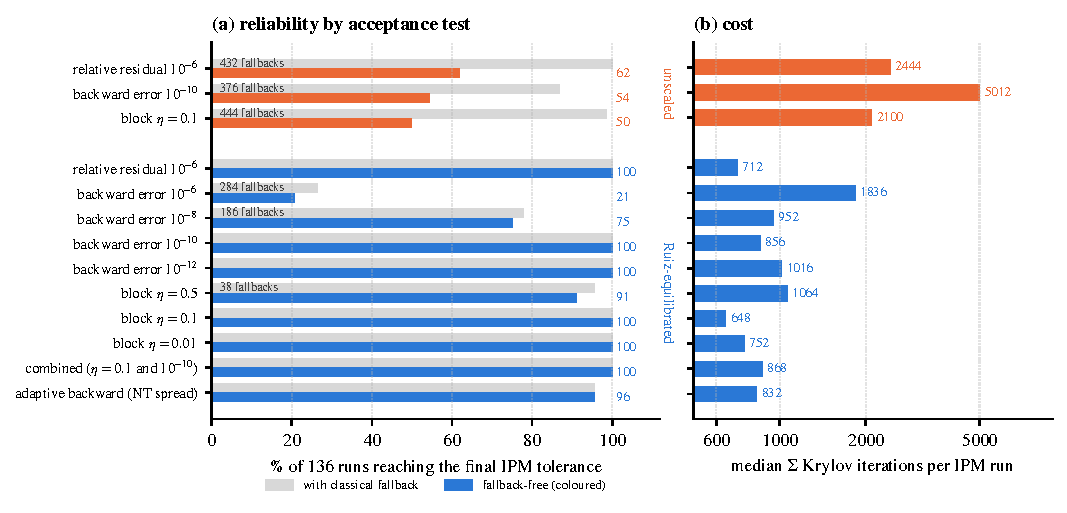
\includegraphics[width=\textwidth]{fig_criteria.pdf}
\caption{Acceptance-test ablation (Table~\ref{tab:criteria}). (a) Share of the 136 runs reaching the final IPM tolerance with classical fallback (grey) and without it (coloured; numbers at the bar ends); (b) median Krylov work per run. Red: unscaled; blue: Ruiz-equilibrated.}\label{fig:criteria}
\end{figure}

\subsection{Conditioning and Krylov work along the IPM run}\label{sec:spectrum}
Fig.~\ref{fig:spectrum} follows one IPM run on \ds{sparse\_banded\_n800\_k3\_s1} ($N=2\,480$, session A) with every $\Kt(W)$ and right-hand side captured.

\lead{The equilibrated system remains well conditioned.} The NT spread $\max w/\min w$ grows from $1$ to $1.4\times10^{6}$, whereas $\kappa(D\Kt D)$ stays between $80$ and $178$ (panel a), as Proposition~\ref{prop:cond} predicts. The same capture on \ds{sparse\_banded\_n800\_k3\_s4} in session M gives $\kappa(D\Kt D)$ between $111$ and $703$ at an NT spread of up to $3.5\times10^{5}$; on all \ds{sparse\_banded} instances on which it was measured, the equilibrated condition number stays below about $7\times10^{2}$.

\lead{The iteration count is governed by the eigenvalue distribution.} MINRES iterations nevertheless grow from 92 to $1\,880$ per IPM iteration (panel b), because the share of eigenvalues within 10\,\% of $\pm1$ falls from 76\,\% to 54\,\% and up to 38 eigenvalues of magnitude below $0.1$ appear. Two further measurements are relevant. After the first IPM iteration the combined test costs $1.17$--$1.56\times$ the iterations of the backward-error test alone, and in every solve the binding block is the equality block $y$, whose right-hand side is of order $10^{-15}$ once the iterates are feasible (Section~\ref{sec:accept}). The matrix-free reduced system needs $0.57\times$ the iterations early in the run but $2.8\times$ late in the run, which confirms the augmented system as the appropriate target.

\lead{Deflation would help; harvested recycling does not.} Panel (c) bounds what deflation could achieve: exact removal of the $k$ smallest-magnitude eigenpairs reduces the iterations $1.7\times$ ($k=10$), $3.7\times$ ($k=50$) and $6.2\times$ ($k=100$). A recycled-MINRES prototype, with harmonic Ritz vectors harvested from the Lanczos process ($k=40$--$80$) and carried across the solves of one run, achieved only $1.38$--$1.63\times$ fewer iterations at $6\times$ the CPU time, because the harvested vectors approximate the interior eigenvalues poorly; it was not adopted.

\begin{figure}[t]\centering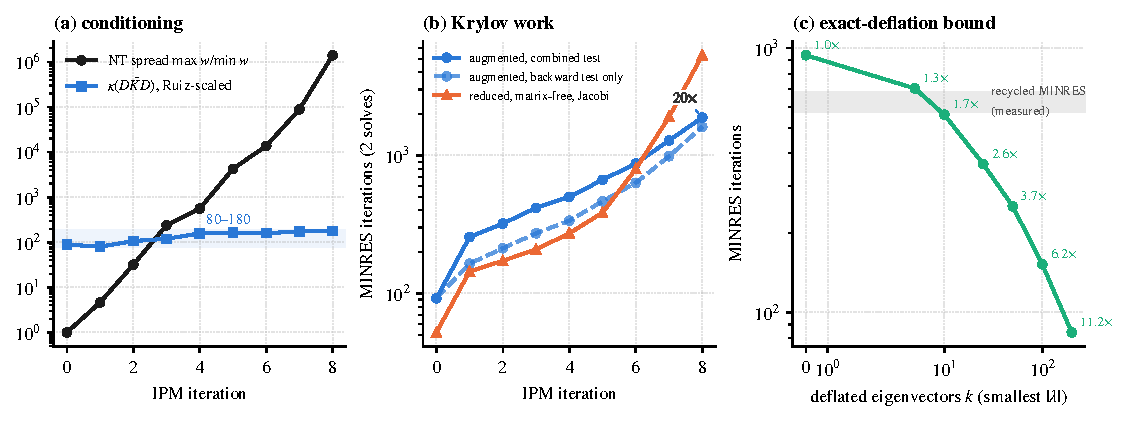
\includegraphics[width=\textwidth]{fig_spectrum.pdf}
\caption{One captured IPM run on \ds{sparse\_banded\_n800\_k3\_s1} ($N=2\,480$). (a) The NT scaling spreads over six orders of magnitude while $\kappa$ of the Ruiz-equilibrated KKT matrix stays below 180. (b) MINRES iterations for the two solves of each IPM iteration under the combined test, under the backward-error test alone, and on the matrix-free reduced system. (c) Iterations at the last IPM iteration after exact deflation of the $k$ smallest-$|\lambda|$ eigenpairs (an upper bound for any recycling scheme); the grey band marks what the recycled-MINRES prototype achieved.}\label{fig:spectrum}
\end{figure}

\subsection{Scaling behaviour}\label{sec:scaling}
Table~\ref{tab:scaling} and Fig.~\ref{fig:scaling} report the whole-run wall time on the two sparse families (session M; five instances per size on \ds{sparse\_banded} up to $N=9\,920$).

\lead{Cost.} On \ds{sparse\_banded}, the direct solvers scale like $N^{2.3}$ (LDL$\T$) and $N^{1.9}$ (CHOLMOD) over the measured range and like $N^{3.2}$--$N^{3.5}$ between the two largest sizes they completed; the predictive budget stopped them beyond $N=19\,840$. Equilibrated MINRES on the CPU scales like $N^{1.2}$, because its total Krylov iteration count grows like $N^{0.55}$ (from $1\,500$ to $39\,000$ per run).

\lead{Crossover.} MINRES is slower than the sparse LDL$\T$ factorisation below $N\approx5\,000$ ($0.06\times$ at $N=310$), breaks even at $N=4\,960$ (paired ratio $1.26$; $0.97$--$1.47$ over five instances), and is $3.5\times$ ($3.1$--$4.5\times$) faster at $N=9\,920$ and $9.4\times$ ($8.5$--$10.3\times$, two instances) at $N=19\,840$, where it also outperforms the CHOLMOD-based reduced solver by $13\times$. The instance-to-instance spread is below $\pm30\,\%$ at every size beyond $N=1\,240$.

\lead{Low-fill control.} On \ds{sparse\_lowfill} the direct solvers win at every size up to $N=39\,680$ (the reduced CHOLMOD solve is $1.9$--$5.2\times$ faster than CPU MINRES from $N=4\,960$ on); only at $N=79\,360$ does GPU MINRES overtake both direct solvers ($3.7\times$), where the dense $p\times p$ Schur complement of the reduced solver and the LDL$\T$ factorisation both become expensive. The speed-up on \ds{sparse\_banded} is therefore a statement about fill-in, not about iterative methods in general.

\lead{Memory.} Fill-in costs memory as well as time (Fig.~\ref{fig:scaling}c): at $N=19\,840$ on \ds{sparse\_banded}, resident memory grows during a run by 390\,MB (LDL$\T$), 472\,MB (lazy refactorisation) and 722\,MB (CHOLMOD), against 47\,MB for CPU MINRES; at $N=79\,360$, CPU MINRES needs 218\,MB and GPU MINRES 134\,MB of device memory. On \ds{sparse\_lowfill} the direct solvers are frugal up to $N=19\,840$ but grow by 287\,MB (LDL$\T$) and $2.6$\,GB (CHOLMOD with the dense Schur complement) at $N=79\,360$. Below $N\approx5\,000$ the growth is below the sampling resolution because Python's allocator reuses memory between runs.

\lead{Performance profiles.} Fig.~\ref{fig:profiles}(a,b) aggregates all 57 sparse instances. On \ds{sparse\_banded}, LDL$\T$ is the fastest method on 56\,\% of the instances (the small ones) but solves only 89\,\% within the budget; CPU MINRES and the automatic CPU/GPU dispatch solve all of them, and the dispatch is within $2\times$ of the fastest method on 50\,\%. On \ds{sparse\_lowfill}, LDL$\T$ is within $2\times$ of the fastest on 95\,\% of the instances and CPU MINRES on 5\,\%.

\lead{Replication.} Sessions B--E reproduce every crossover (Appendix~\ref{app:replication}): the MINRES/LDL$\T$ ratio at $N=9\,920$ is $3.9$, $3.1$, $4.0$ and $4.1\times$ in sessions B, C, D and E, at $19\,840$ it is $9.1$, $9.5$ and $9.1\times$ in sessions B, C and E, and the GPU/CPU ratio at $79\,360$ is $3.7\times$ in both GPU replications.

\begin{table}[t]\centering\small
\caption{Median wall time [s] of the whole IPM run (session M; per instance the median of two repetitions, then the median over the instances of a size). Empty: skipped by the predictive budget ($>450$\,s predicted) or above the exact-LU limit. Last column: median and range over instances of the paired ratio LDL$\T$/MINRES on the CPU (latency-optimised kernel).}\label{tab:scaling}
\resizebox{\textwidth}{!}{%
\begin{tabular}{r|rrr|rr|rr|l}\toprule
 & \multicolumn{3}{c|}{direct} & \multicolumn{2}{c|}{MINRES, latency-optimised} & \multicolumn{2}{c|}{MINRES, baseline kernel} & LDL$\T$/MINRES\\
$N$ & LDL$\T$ & reduced & lazy refact. & CPU & GPU & CPU & GPU & CPU\\\midrule
\inputrows{tex/scaling_rows.tex}\bottomrule
\end{tabular}}
\end{table}

\begin{figure}[t]\centering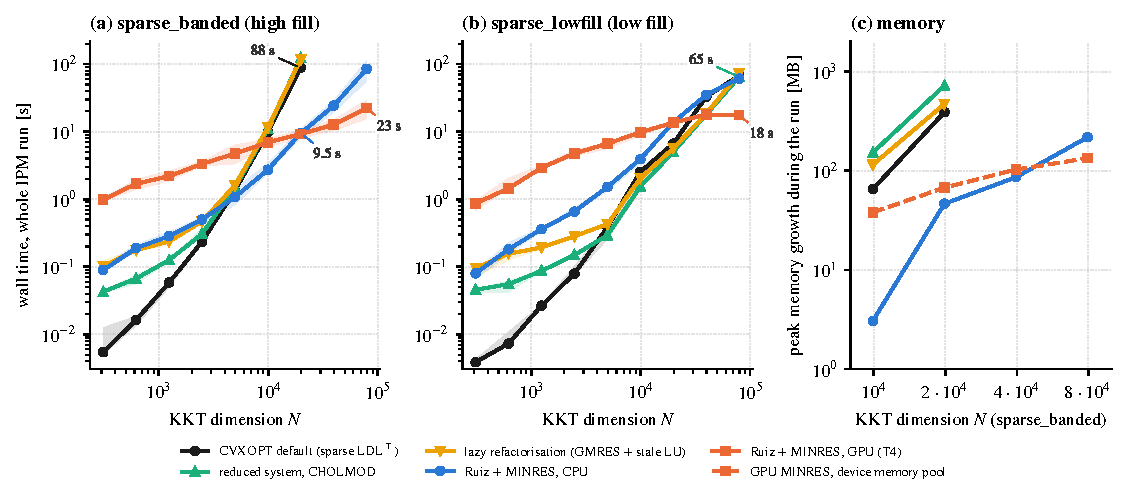
\includegraphics[width=\textwidth]{fig_scaling.pdf}
\caption{(a, b) Whole-run wall time versus KKT dimension (Table~\ref{tab:scaling}); bands: range over the instances of a size. The iterative methods win under high fill-in (a) and lose under low fill-in (b) except at the largest size on the GPU. (c) Growth of resident memory during the run on \ds{sparse\_banded}, and the CuPy device-memory pool of GPU MINRES.}\label{fig:scaling}
\end{figure}

\begin{figure}[t]\centering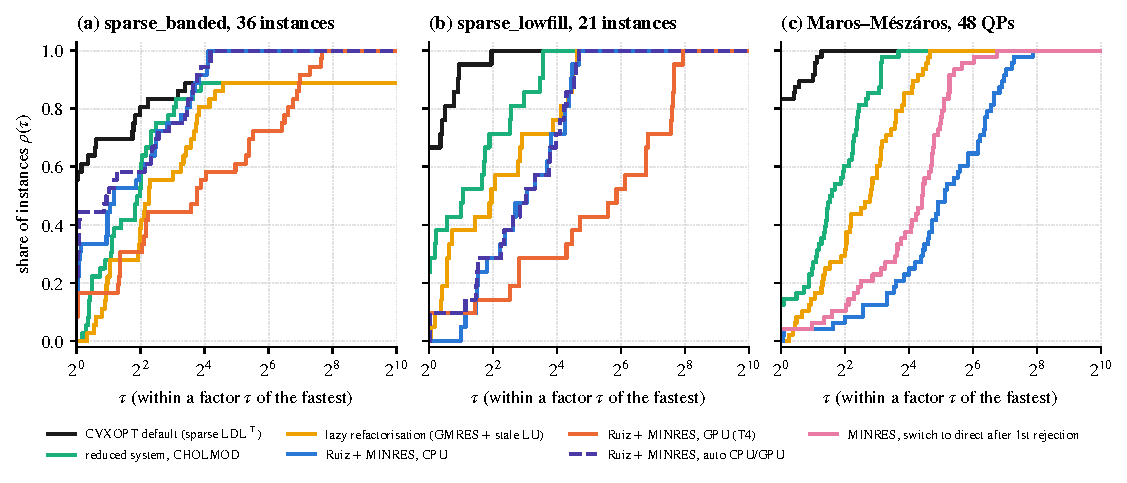
\includegraphics[width=\textwidth]{fig_profiles.pdf}
\caption{Performance profiles~\cite{dolan2002benchmarking} of whole-run wall time (session M): $\rho(\tau)$ is the share of instances on which a method reaches the final tolerance within $\tau$ times the time of the fastest method on that instance; runs skipped by the budget count as unsolved. (a, b) Synthetic sparse families; (c) Maros--M\'esz\'aros QPs (Section~\ref{sec:realqp}).}\label{fig:profiles}
\end{figure}

\subsection{GPU kernel}\label{sec:gpu}
Fig.~\ref{fig:gpu} isolates the kernel.

\lead{The baseline kernel is latency-bound.} The GPU sparse mat-vec takes a constant $\approx0.07$\,ms at every size and is $13.4\times$ faster than the CPU at $N=79\,360$ (panel a, dotted), but the baseline kernel spends $0.68$--$0.73$\,ms per MINRES iteration independently of $N$---about $90\,\%$ of its time in synchronisation and launch overhead, in agreement with~\eqref{eq:latency}.

\lead{The latency-optimised kernel.} The kernel of Section~\ref{sec:gpumodel} costs $0.53$--$0.62$\,ms per iteration and is $1.14$--$1.29\times$ faster than the baseline kernel at every size on the GPU, and up to $1.21\times$ faster on the CPU, where the gain comes from the CSR-level equilibration sweep and the sparser checks (it is $15\,\%$ slower at $N=310$). Its Krylov iteration count is within $3.5\,\%$ of that of the baseline kernel (the adaptive checks overshoot slightly), and it is fallback-free on every run. The whole-run GPU speed-up over the CPU is $1.02\times$ at $N=19\,840$, $1.90\times$ at $39\,680$ and $3.75\times$ ($3.62$--$3.87\times$) at $79\,360$ (panel b); below $N\approx10^{4}$ the GPU is slower. The automatic dispatch at $N=2\times10^{4}$ therefore uses the CPU up to $19\,840$ and the GPU beyond, and is the fastest MINRES variant at every size (Fig.~\ref{fig:profiles}a).

\lead{Mixed precision does not help here.} Single-precision MINRES inside double-precision refinement, evaluated offline, needs $1.36\times$ more iterations, because each restart discards the Krylov space, which a latency-bound kernel cannot recover.

\begin{figure}[t]\centering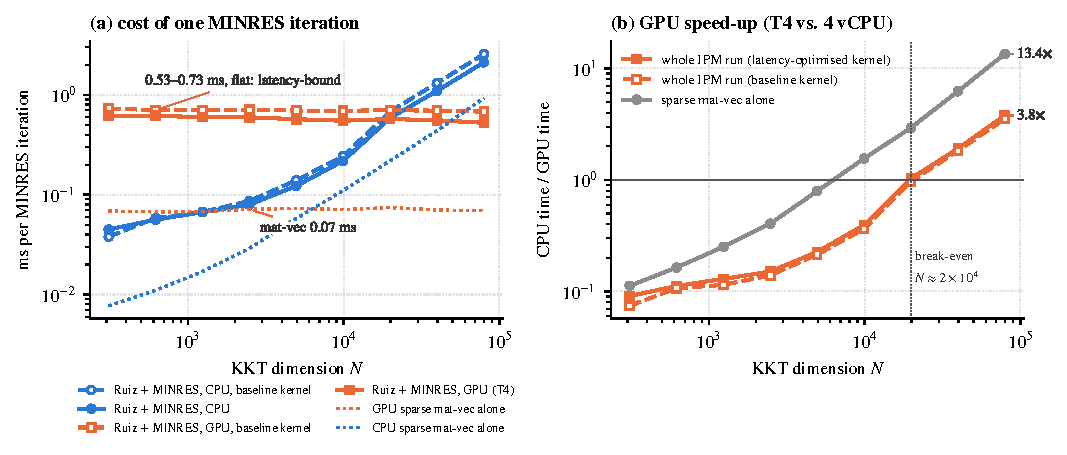
\includegraphics[width=\textwidth]{fig_gpu.pdf}
\caption{GPU kernel on a Tesla T4 (session M). (a) Milliseconds per MINRES iteration (solve and acceptance checks) for the baseline (dashed) and latency-optimised (solid) kernels on CPU and GPU, with the sparse mat-vec alone (dotted). (b) Speed-up of the GPU over the 4-vCPU host for the whole IPM run and for the mat-vec alone.}\label{fig:gpu}
\end{figure}

\subsection{Real-world QPs}\label{sec:realqp}
Table~\ref{tab:mm}, Fig.~\ref{fig:realqp} and Fig.~\ref{fig:profiles}(c) report the 48 Maros--M\'esz\'aros instances (session M).

\lead{Every method is accurate; the direct solver is fastest.} All methods reach the independent tolerances on every instance, with objective values within $6.3\times10^{-9}$ of those of the unmodified solver and, on 46 of 48 instances, the same IPM iteration count. However, \textsc{cvxopt}'s own LDL$\T$ factorisation is the fastest method on 40 instances, the reduced CHOLMOD solve on 6, and a MINRES variant on 2 (\ds{GOULDQP3} and \ds{PRIMAL4}, where MINRES needs no fallback). Equilibrated MINRES is a median $31\times$ slower than LDL$\T$, and its performance profile reaches $\rho=0.25$ only at $\tau=16$.

\lead{The equilibrated matrices are ill-conditioned.} MINRES needs classical fallback on 26 instances (403 of its $1\,520$ solves). An offline diagnostic on eight instances with $N\le1\,565$ (Fig.~\ref{fig:realqp}b, Table~\ref{tab:equil}) recorded $\kappa(D\Kt D)$ along the run: it reaches $2.4\times10^{6}$ (\ds{QE226}) to $4.2\times10^{15}$ (\ds{QSC205}) on the five instances that need fallback, where MINRES reaches its iteration cap, and stays between $7.3\times10^{2}$ (\ds{DUAL1}) and $1.0\times10^{7}$ (\ds{CVXQP1\_S}) on the three that do not, against at most about $7\times10^{2}$ on \ds{sparse\_banded}. These problems violate the premises of Proposition~\ref{prop:cond}---$P$ is singular on 18 of the 48 and the active sets are degenerate---so the boundedness that makes equilibration sufficient on the synthetic families does not hold, and an unpreconditioned Krylov method stalls.

\lead{Switching to the direct solver limits the damage but does not close the gap.} Using MINRES until its first rejected direction and the direct solver thereafter reduces the fallbacks from 403 to 43 and the total MINRES time from 721\,s to 214\,s (median per instance from $3.2$ to $0.86$\,s), while MINRES still delivers 63\,\% of all KKT solves (median 80\,\% per instance). It remains a median $21\times$ slower than LDL$\T$. Its 16 rejected directions are directions of the full-matrix LU decomposition used after the switch that miss the backward-error test at $\kappa$ up to $10^{15}$.

\lead{The GPU does not help at these sizes.} On the eleven instances with $2\,400\le N\le3\,962$ on which it ran, GPU MINRES is $1.9$--$8.8\times$ (median $7.4\times$) slower than CPU MINRES with the same Krylov counts, as the latency model predicts below $N\approx2\times10^{4}$; the budget stopped it beyond $N=3\,962$.

\begin{table}[t]\centering\small
\caption{Maros--M\'esz\'aros QPs (48 instances, $N=91$--$10\,192$, session M). \emph{strict}: tolerances reached without fallback or rejected direction; \emph{inst.\,fb}: instances with at least one fallback; \emph{same its}: share of instances with the IPM iteration count of the unmodified solver; speed-up: median over instances of the paired ratio to the unmodified LDL$\T$; fastest: number of instances on which the method was the fastest of the five CPU methods.}\label{tab:mm}
\resizebox{\textwidth}{!}{%
\begin{tabular}{lrrrrrrrrr}\toprule
method & inst. & strict\,\% & inst.\,fb & fallbacks & same its\,\% & median [s] & total [s] & speed-up & fastest\\\midrule
\inputrows{tex/mm_rows.tex}\bottomrule
\end{tabular}}
\end{table}

\begin{figure}[t]\centering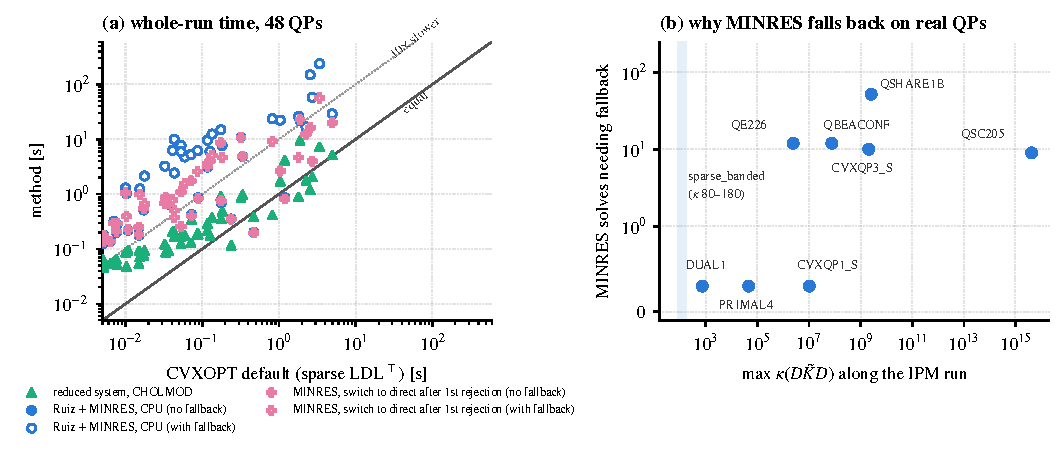
\includegraphics[width=\textwidth]{fig_realqp.pdf}
\caption{Maros--M\'esz\'aros QPs. (a) Whole-run time of three methods against \textsc{cvxopt}'s LDL$\T$ on the 48 instances; hollow markers: at least one classical fallback. (b) Offline diagnostic on eight instances: the largest condition number of the Ruiz-equilibrated KKT matrix along the IPM run against the number of MINRES solves that needed fallback; the band marks \ds{sparse\_banded}.}\label{fig:realqp}
\end{figure}

\subsection{The precision requirement of a Newton direction}\label{sec:noise}
Two experiments quantify the requirement that any inexact or quantum solver must meet (Fig.~\ref{fig:noise}).

\lead{Injected direction error.} The exact direction is perturbed by a random relative error of prescribed size before it is returned to the IPM (no acceptance test, no fallback). With an isotropic relative error of $10^{-7}$ or $10^{-8}$, all 15 instances reach the final tolerance in the usual 6--7 iterations; with $10^{-6}$ none does within 100 iterations, and block-wise relative errors of $10^{-3}$ or larger fail as well. The threshold coincides with \textsc{cvxopt}'s own tolerance of $10^{-7}$: the IPM cannot converge below the accuracy of its directions.

\lead{The requirement scales with the IPM tolerance.} Table~\ref{tab:tolsweep} and Fig.~\ref{fig:noise}(b) repeat the experiment on 30 dense instances with \textsc{cvxopt}'s tolerances set to $\tau\in\{10^{-8},10^{-6},10^{-4}\}$ (absolute and feasibility tolerance $\tau$, relative tolerance $10\tau$) and the acceptance thresholds scaled accordingly (primal and dual residuals $\le10\tau$, gap and objective error $\le100\tau$; $\tau=10^{-7}$ recovers the defaults). The largest isotropic error tolerated on every instance is $10^{-7}$ at $\tau=10^{-6}$ and $10^{-5}$ at $\tau=10^{-4}$, and $10^{-8}$ is tolerated on 29 of 30 instances at $\tau=10^{-8}$---between $\tau/10$ and $\tau$ at every level. Block-wise errors of $10^{-3}$ are tolerated only at $\tau=10^{-4}$, and then on 27\,\% of the instances. The combined-test MINRES reaches every tolerance with the iteration count of the unmodified solver. The precision a KKT solver must deliver is therefore set by the optimisation tolerance, which is the quantity to budget for when a quantum or other inexact solver is costed (Corollary~\ref{cor:precision}).

\begin{table}[t]\centering\small
\caption{Share of 30 dense instances [\%] reaching the final tolerance when every Newton direction carries an injected relative error $\delta$, at IPM tolerance $\tau$ (session M; the $\tau=10^{-7}$ column is the injected-error experiment at \textsc{cvxopt}'s defaults on 15 instances). Solver rows: share and, in parentheses, median IPM iterations.}\label{tab:tolsweep}
\begin{tabular}{llrrrr}\toprule
error model & $\delta$ & $\tau=10^{-8}$ & $\tau=10^{-7}$ & $\tau=10^{-6}$ & $\tau=10^{-4}$\\\midrule
\inputrows{tex/tolerance_rows.tex}\bottomrule
\end{tabular}
\end{table}

\lead{Optimisation-level refinement.} Following~\cite{gleixner2016ir}, the QP is solved to a loose tolerance of $10^{-3}$, the problem is shifted and scaled around the current point, and the correction QP is solved again, five times. With exact inner solves, or with MINRES accepted at a backward error of $10^{-4}$, the error on the original problem falls from $1.7\times10^{-4}$ to $5\times10^{-9}$, $5\times10^{-13}$ and $10^{-15}$ (9/9 instances below $10^{-7}$); with an injected forward error of $10^{-4}$ or $10^{-3}$ it stalls (2/9 and 1/9 instances), and with HHL directions without fallback it stalls as well (1/3 and 0/3). The correction QPs are badly conditioned---in session M, which also records the equilibrated condition number, their KKT matrices reach $\kappa(D\Kt D)=7\times10^{6}$ in the median and $10^{10}$ at most in the MINRES runs---yet residual-controlled MINRES still converges. Outer refinement thus relaxes the \emph{residual} accuracy that a classical iterative solver must reach inside the IPM, but it does not make a forward-error-limited solver sufficient.

\begin{figure}[t]\centering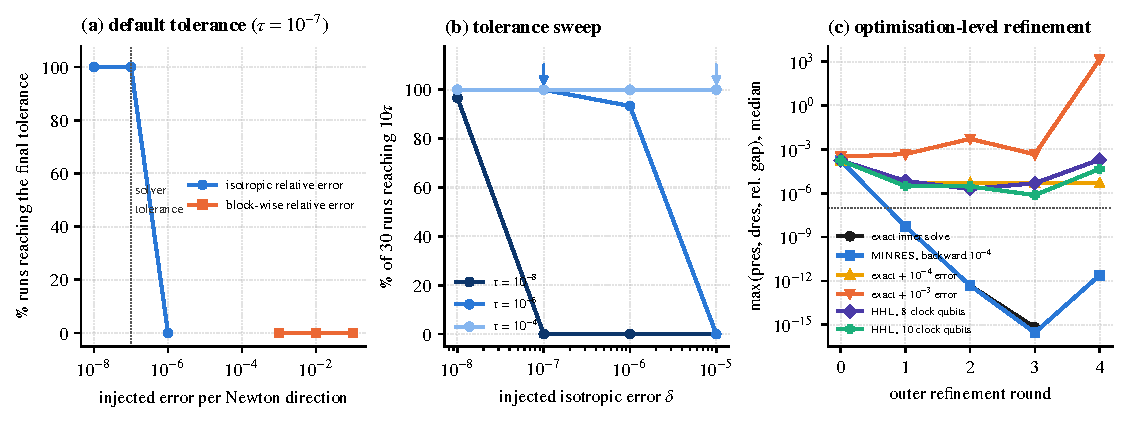
\includegraphics[width=\textwidth]{fig_noise_outer.pdf}
\caption{(a) Share of IPM runs reaching the final tolerance when every Newton direction carries an injected relative error, at \textsc{cvxopt}'s default tolerance (15 instances). (b) The same for isotropic error at three IPM tolerances $\tau$ (30 instances); arrows mark the largest error tolerated on every instance. (c) Optimisation-level iterative refinement with different inner KKT solvers (session A; medians over 9 instances, HHL: 3; dotted: $10^{-7}$).}\label{fig:noise}
\end{figure}

\subsection{Alternatives evaluated and not adopted}\label{sec:notadopted}
Table~\ref{tab:notadopted} lists the alternatives that were implemented or prototyped and the measurement that led us not to adopt them. The most instructive negative results concern the reduced target system (Section~\ref{sec:spectrum}), recycled MINRES and randomised Nystr\"om preconditioning~\cite{chu2026nystrom}: on our families the effective dimension of the active-constraint term $\Ghat\T\Ghat$ equals the number of active constraints ($480$ of $n=800$), and removing even the 100 dominant eigenpairs of $S$ leaves $\kappa(S)=1.5\times10^{5}$, so the low-rank premise fails. The method should suit problems with few active constraints (e.g.\ portfolio selection or support-vector machines), which we have not tested.

\begin{table}[t]\centering\small
\caption{Alternatives evaluated and not adopted (measured on the benchmark of Section~\ref{sec:setup} or on its captured KKT sequences).}\label{tab:notadopted}
\begin{tabularx}{\textwidth}{p{5.2cm}X}\toprule
method & measurement\\\midrule
warm start of the combined solve from the affine direction & $\le4\,\%$ fewer Krylov iterations on sparse, more on dense instances; a naive variant accepts the affine direction itself under $\eta=0.1$ and diverged on 2/35 instances\\
switch to the exact solver after the first rejected direction & never triggered on the synthetic families; on the Maros--M\'esz\'aros collection it reduces fallbacks from 403 to 43 and time $3.4\times$ but remains $21\times$ slower than LDL$\T$ (Section~\ref{sec:realqp})\\
CG on the null-space system~\eqref{eq:oss} (dense basis) & $2.1\times$ fewer Krylov iterations than augmented MINRES on the dense families, $0.65$--$1.24\times$ on the sparse families; the dense basis makes it $23$--$29\times$ slower at $N=9\,920$\\
lazy refactorisation (GMRES + stale factorisation) & half of the factorisations saved on small instances, none at scale (the scaling changes too fast); same cost as the direct solver at $N=19\,840$\\
reduced system, matrix-free, Jacobi-scaled & $0.57\times$ the iterations early, $2.8\times$ late in the run\\
square-root system $B=[L\T;\Ghat]$ with LSQR & $\kappa(B)=\sqrt{\kappa(S)}$ helps only when $\kappa(P)$ dominates; loses late in the run\\
recycled MINRES (harmonic Ritz, $k=40$--$80$) & $1.38$--$1.63\times$ fewer iterations, $6\times$ more CPU time (exact-deflation bound: $3.7$--$6.2\times$)\\
randomised Nystr\"om preconditioning & effective dimension of $\Ghat\T\Ghat$ equals the number of active constraints ($0.6n$); rank-100 removal leaves $\kappa(S)=1.5\times10^{5}$\\
single-precision MINRES + double-precision refinement & $1.36\times$ more iterations (Krylov space discarded at each restart)\\
relaxed block floor $\phi_b$ ($10^{-9}\to10^{-8}$) & $6\,\%$ fewer iterations on 51 instances (a tolerance relaxation, not adopted as default)\\
dequantised (sampling-based) solver~\cite{tang2019dequantize} & $99\,\%$ of the singular directions needed for 30\,\% accuracy; stable rank $0.13N$: no low-rank structure to exploit\\\bottomrule
\end{tabularx}
\end{table}

\section{Results: quantum solvers}\label{sec:quantum}
\subsection{Setup and scope of the simulation}\label{sec:qsetup}
All results in this section are classical statevector simulations of ideal circuits with oracle block encoding and state preparation; they establish algorithmic feasibility and relative cost, not a speed-up over classical solvers. The captured KKT systems are equilibrated matrices from the \ds{sanity} and dense families and from SDPLIB ($N\le64$, padded to $2^{n_d}$), and the integrated runs use eight instances inside \texttt{coneqp}: \ds{tiny\_A}, \ds{tiny\_B}, \ds{tiny\_C}, \ds{dense\_noeq\_n10\_k0\_s0}, \ds{dense\_kappa\_n10\_k0\_s0}, \ds{dense\_kappa\_n10\_k0\_s1}, \ds{dense\_kappa\_n10\_k3\_s0} and \ds{dense\_kappa\_n10\_k3\_s1} ($N\le32$). The walk-level simulation of the polynomial solver is cross-checked in three ways: the identity $\Pi\mathcal W^k\Pi=T_k(\Kh)$ is asserted numerically; an explicit index-register statevector agrees with the accumulated form to $10^{-16}$; and the cached spectral evaluation used for the second right-hand side and the refinement rounds agrees with the walk simulation to within $10^{-11}$ on every system (logged per solve). A simulation cap of $4\times10^{5}$ walk steps makes circuits beyond the budget fail with an explicit label; no classical result is ever substituted. The polynomial experiments on captured systems (Sections~\ref{sec:qpoly} and~\ref{sec:qcost}) come from session A; the HHL accuracy study, the integrated runs, the sampling-seed sweep and the null-space study from session M, in which the statevector simulator runs on the GPU. Because instances, matrices and quantum samples are seeded deterministically, every integrated configuration has the same strict-success count in sessions A, M and E.

\subsection{HHL: accuracy and behaviour inside the IPM}\label{sec:hhl}
Fig.~\ref{fig:qaccuracy}(a) shows the forward error of the HHL output with ideal readout on 20 captured systems---five IPM iterations each of \ds{tiny\_A}, \ds{tiny\_B}, \ds{tiny\_C} and the SDPLIB instance \ds{truss1}, with $\kappa(\Kt)$ from $2.0$ to $7.4\times10^{10}$---as a function of the clock register. Without scaling, the median error is $\ge0.9$ up to 6 clock qubits and $1.5$--$2.7\times10^{-2}$ at 10; Ruiz equilibration reduces it to $4.6\times10^{-3}$ ($\kappa$-known mode) and $1.2\times10^{-3}$ (resolution mode) at 10 clock qubits---four orders of magnitude short of the $10^{-7}$ required by the IPM (Section~\ref{sec:noise}). Finite-shot readout adds error: at 10 clock qubits with equilibration, the median error is $1.8\times10^{-2}$ ($\kappa$-known) and $0.15$ (resolution) with $10^{5}$ accepted samples per setting, and $3.3\times10^{-2}$ and $0.55$ with $10^{6}$ raw shots. Inside the IPM (Table~\ref{tab:integrated}), with a budget of 4 refinement rounds per solve, HHL without fallback is strict on at most one of the three \ds{sanity} instances per configuration (\ds{tiny\_B}, $N=8$, $\kh\le84$, at $n_c=8$) and forces the IPM to use between 64 and 179 rejected directions per configuration; 12 clock qubits add no success. Regularising the scaled system by $\delta I$ lowers $\kappa$ but limits refinement to a residual of about $\delta$, and the block test alone diverges on SDPLIB, so neither is a remedy.

\begin{figure}[t]\centering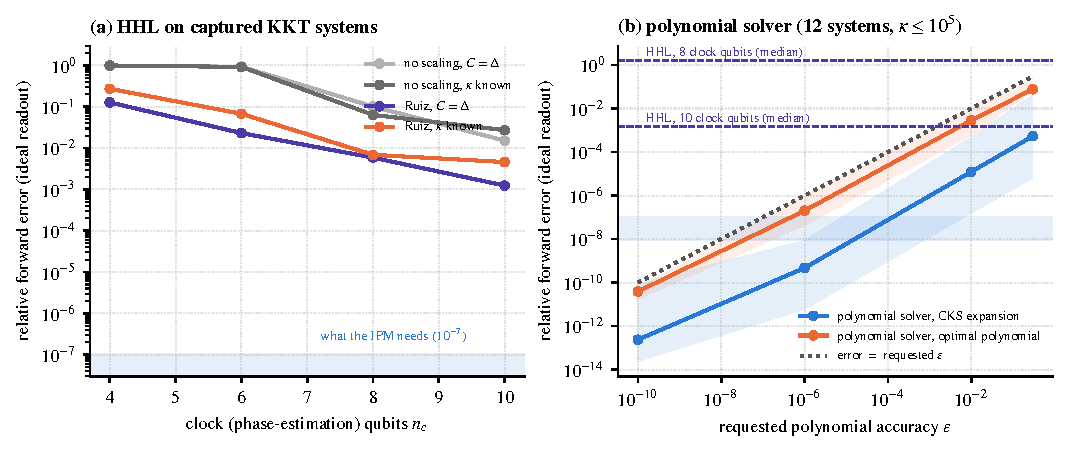
\includegraphics[width=\textwidth]{fig_qaccuracy.pdf}
\caption{Forward error of quantum linear solvers on captured KKT systems with ideal (statevector) readout. (a) HHL versus clock-register size for the four scaling and reciprocal variants (medians over 20 systems, session M). (b) Polynomial solver versus requested accuracy $\eps$ for the CKS expansion and the optimal polynomial (medians and min--max over 12 systems, session A); the CKS bound over-delivers by 3--4 orders of magnitude, whereas the optimal polynomial sits at the target. The shaded band marks the $10^{-7}$ requirement of Section~\ref{sec:noise}.}\label{fig:qaccuracy}
\end{figure}

\subsection{Polynomial solver: accuracy and degree}\label{sec:qpoly}
Fig.~\ref{fig:qaccuracy}(b) shows that the forward error of the polynomial solver follows the requested $\eps$: $2.4\times10^{-13}$ (CKS) and $3.9\times10^{-11}$ (optimal) at $\eps=10^{-10}$, and $4.7\times10^{-10}$ and $2.0\times10^{-7}$ at $\eps=10^{-6}$. On the 38 (system, $\eps$) pairs on which both polynomials ran, the optimal polynomial needs $2.70\times$ fewer walk steps (range $2.26$--$3.36$) and has a $1.89\times$ higher success probability, i.e.\ $4.8\times$ fewer walk steps per successful sample (Table~\ref{tab:poly}, Fig.~\ref{fig:poly}). Eight of the 96 configurations (four per polynomial) exceeded the simulation cap ($\kappa\ge2\times10^{4}$) and are reported as not run, never as successes.

\begin{table}[t]\centering\small
\caption{Degree $d$ (walk steps, i.e.\ block-encoding queries per circuit) and LCU 1-norm $\norm{c}_1$ of the two inversion polynomials at equal target accuracy $\eps$ on $\mathcal D_\kappa$. Cost ratio $=(d_{\text{CKS}}/d_{\text{opt}})\,(\norm{c}_1^{\text{CKS}}/\norm{c}_1^{\text{opt}})^2$ (walk steps per successful sample).}\label{tab:poly}
\begin{tabular}{rr|rr|rr|rr}\toprule
$\kappa$ & $\eps$ & $d_{\text{CKS}}$ & $d_{\text{opt}}$ & $\norm{c}_1^{\text{CKS}}$ & $\norm{c}_1^{\text{opt}}$ & $d$ ratio & cost ratio\\\midrule
\inputrows{tex/poly_rows.tex}\bottomrule
\end{tabular}
\end{table}

\begin{figure}[t]\centering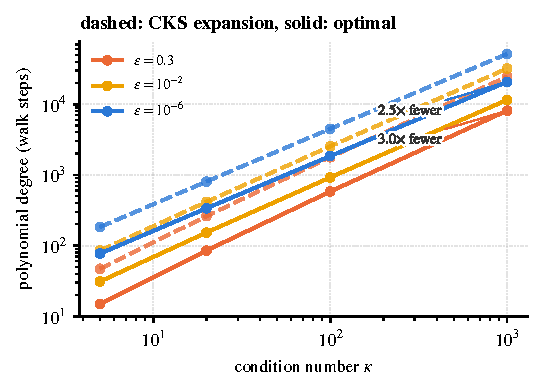
\includegraphics[width=0.5\textwidth]{fig_poly.pdf}
\caption{Degree of the two inversion polynomials versus $\kappa$ at three target accuracies (Table~\ref{tab:poly}).}\label{fig:poly}
\end{figure}

\subsection{Cost of refinement: precision versus samples}\label{sec:qcost}
The cost model~\eqref{eq:qcost} predicts that the cheapest way to reach a given final residual is a low-precision circuit with few samples per round. Fig.~\ref{fig:qcost} and Table~\ref{tab:qcost} test this prediction on 9 captured systems ($\kh\le4.3\times10^{3}$) refined to a residual of $10^{-10}$ with finite-shot readout under emulated amplitude amplification. Every configuration in the table converged on every system (the optimal polynomial at $\eps=10^{-6}$ exceeded its generation cap on one or two systems and is omitted).

\lead{Low precision and few samples are cheapest.} Relative to a high-precision baseline---the CKS expansion at $\eps=10^{-6}$ with $20\,000$ samples per round---the paired median reduction in block-encoding queries is $20\times$ from using 500 samples per round alone, $237\times$ with the optimal polynomial at $\eps=0.3$ and 500 samples, and $624\times$ at 200 samples, at the price of 20 instead of 7 refinement rounds.

\lead{The contraction rate is set by the larger of two error sources.} With the accurate CKS circuit, the contraction per round is set by the sampling error ($0.22$, $0.15$, $0.10$, $0.043$ and $0.018$ at $200$, $500$, $10^{3}$, $4\times10^{3}$ and $2\times10^{4}$ samples per round), in agreement with $c_0\sqrt{N/(2S)}$; with the $\eps=0.3$ circuit it saturates at $0.25$--$0.30\approx\eps$ regardless of the sample count. The readout contribution does not depend measurably on $\kh$ (Remark~\ref{rem:readout}), so the conditioning enters the cost through the circuit depth and the post-selection probability, not through the number of rounds.

\begin{table}[t]\centering\small
\caption{Cost of refining a finite-shot solve to a residual of $10^{-10}$ on 9 captured KKT systems (medians, session A). \emph{queries} $=$ rounds $\times$ samples $\times$ walk steps $/\sqrt{p_{\text{succ}}}$ (ideal amplitude amplification). Reduction: paired median ratio to the high-precision baseline in the first row.}\label{tab:qcost}
\begin{tabular}{llrrrrr}\toprule
polynomial & $\eps$ & samples/round & rounds & walk steps & queries & reduction\\\midrule
\inputrows{tex/qcost_rows.tex}\bottomrule
\end{tabular}
\end{table}

\begin{figure}[t]\centering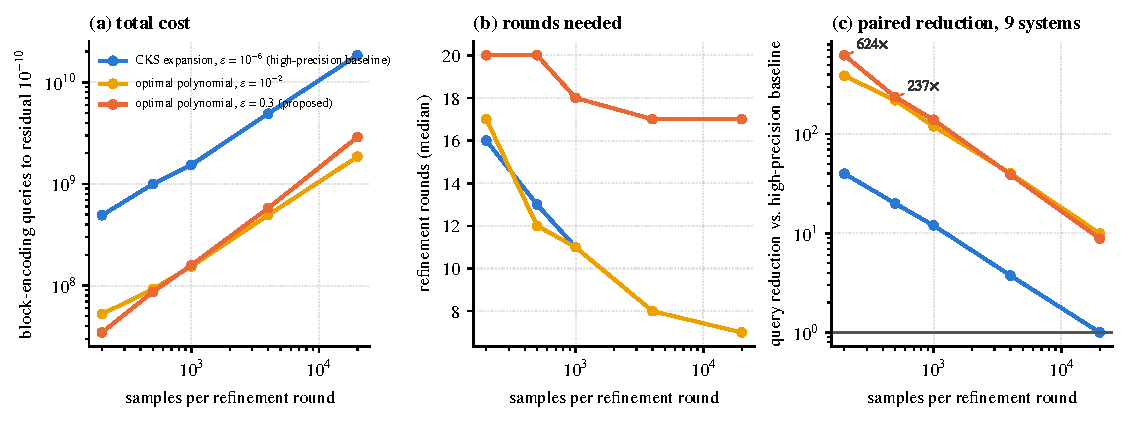
\includegraphics[width=\textwidth]{fig_qcost.pdf}
\caption{Cost of refinement to residual $10^{-10}$ versus samples per round for three (polynomial, $\eps$) settings (9 captured systems, medians, session A). Low circuit precision and few samples per round minimise the total number of block-encoding queries (a) at the expense of more rounds (b); (c) paired reduction relative to the high-precision baseline.}\label{fig:qcost}
\end{figure}

\subsection{Quantum solvers inside the IPM}\label{sec:qintegrated}
Table~\ref{tab:integrated} and Fig.~\ref{fig:qinstances} give the central quantum result: the IPM runs with a simulated quantum KKT solver and \emph{no} classical fallback, and every direction is subject to the combined acceptance test ($\eta=0.1$, $\omega\le10^{-8}$).

\lead{Polynomial solver.} With ideal readout, the solver is strict on 8/8 instances both at high circuit precision ($\eps=10^{-10}$, no refinement needed) and at $\eps=0.3$ with refinement (971 rounds over 90 solves); \textsc{cvxopt} declares \emph{optimal} on 7 and 8 of them, the exception being a run whose next IPM iteration exceeded the depth cap after the independent tolerances had been met. With finite-shot readout, it is strict on 6/8 instances at 250 samples per setting (500 per round) and on 7/8 at $10^{4}$. In the three non-strict augmented runs every solve passed the acceptance test, and the run stopped at the depth cap in the eighth IPM iteration ($\kappa\approx3.8\times10^{4}$, $1.4\times10^{6}$ walk steps); Section~\ref{sec:qshots} explains why these runs need eight iterations instead of five.

\lead{Replication.} Sessions A and E give the same strict counts on all eight instances, and sessions C and D, which run seven of them, give 7/7, 7/7, 5/7 and 6/7 for the four polynomial configurations; session D gives 7/7 and 2/7 for the null-space solver of Section~\ref{sec:oss} (Appendix~\ref{app:replication}). Because the quantum samples are seeded, these sessions test the software path on different machines; the sampling variance is measured in Section~\ref{sec:qshots}.

\lead{HHL under the same refinement budget.} With 60 refinement rounds per solve, HHL is strict on 2 of the 4 instances tried with 10 clock qubits (ideal readout) and fails on the others after using 50 rejected directions. Iterative refinement converges for any solver with residual factor $\xi<1$, and HHL has $\xi<1$ exactly where its clock resolves the spectrum; the polynomial solver satisfies $\xi<1$ by construction (Theorem~\ref{thm:refine}).

\lead{Cost.} The runs with 500 samples per round used $7.7\times10^{5}$ accepted samples and $8.2\times10^{12}$ block-encoding queries in total (with ideal amplitude amplification), and the runs with $2\times10^{4}$ samples per round $1.1\times10^{7}$ samples and $1.4\times10^{15}$ queries---for systems of dimension at most 32 that a classical LU decomposition solves in microseconds. The smallest post-selection probability was $3.7\times10^{-8}$, and the largest circuit needed 29 qubits.

\begin{table}[t]\centering\footnotesize
\caption{Quantum KKT solvers inside \texttt{coneqp} without classical fallback (session M; sessions A and E give identical strict counts). \emph{strict}: independent final tolerances reached, zero fallbacks, no rejected direction used; \emph{opt.}: runs to which \textsc{cvxopt} itself assigns status \emph{optimal}. ``ideal'': statevector readout; ``$S$'': accepted samples per setting and round (emulated amplitude amplification). \emph{walk steps}: median polynomial degree per solve.}\label{tab:integrated}
\resizebox{\textwidth}{!}{%
\begin{tabular}{llcrrrrr}\toprule
solver & readout & inst. & strict & opt. & rejected used & refine rounds & walk steps\\\midrule
\inputrows{tex/integrated_rows.tex}\bottomrule
\end{tabular}}
\end{table}

\begin{figure}[t]\centering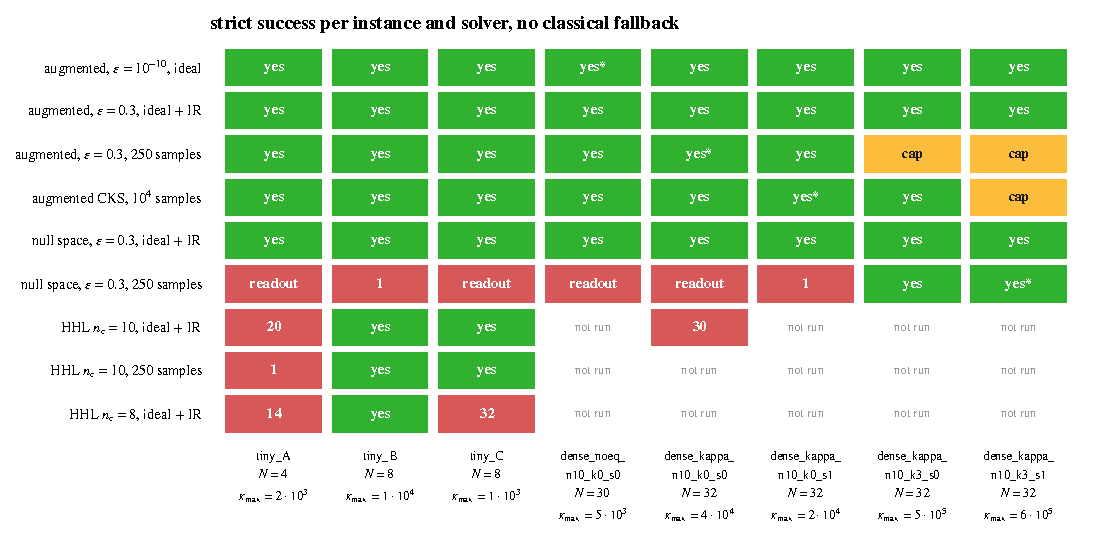
\includegraphics[width=\textwidth]{fig_qinstances.pdf}
\caption{Per-instance outcome of the no-fallback runs with a refinement budget of 60 rounds per solve (session M). Green: strict success; ``yes*'': strict, but \textsc{cvxopt} reports status \emph{unknown} because the depth cap stopped the run after the tolerances had been met. Amber (``cap''): every KKT solve passed the acceptance test, but the run exceeded the simulation's cap of $4\times10^{5}$ walk steps before reaching the tolerances. Red: number of rejected directions the IPM was forced to use, or ``readout'' when the finite-shot reconstruction returned no usable estimate and the run stopped. $\kappa_{\max}$ is the largest condition number of the unscaled KKT matrix encountered in the (strict) ideal-readout polynomial run of that instance.}\label{fig:qinstances}
\end{figure}

\subsection{Sampling seeds and samples per round}\label{sec:qshots}
Each configuration of Table~\ref{tab:integrated} ran with one sampling seed. Table~\ref{tab:shots} and Fig.~\ref{fig:shots} repeat the $\eps=0.3$ polynomial solver on the same eight instances with five sampling seeds at 100, 250, $1\,000$ and $4\,000$ accepted samples per refinement round (both settings together).

\lead{Success depends on the instance, not on the draw.} Strict success rises from 15/40 to 30/40, 30/40 and 39/40. At 100 and 250 samples, every seed gives the same outcome on every instance; the only seed-to-seed variation occurs at $4\,000$ samples (0.88--1.00 per seed). At 100 samples the refinement stalls on the five larger instances, and the IPM is forced to use 65 rejected directions; from 250 samples on no rejected direction is ever used, and every failure is a depth-cap stop on the two instances with $\kappa(P)=10^{3}$ (\ds{dense\_kappa\_n10\_k3\_s0} and \ds{dense\_kappa\_n10\_k3\_s1}).

\lead{Near-threshold directions lengthen the run.} Refinement stops as soon as the combined test holds, so with finite shots the accepted directions have block ratios $\beta$ of $0.03$--$0.06$, close to $\eta=0.1$, whereas with ideal readout the first solve already overshoots the test (median $\beta\approx4\times10^{-3}$, down to $10^{-4}$ on the two $\kappa(P)=10^{3}$ instances). On those two instances, the near-threshold directions cost the IPM three additional iterations (8 instead of 5), which carry it to a barrier parameter at which the KKT matrix reaches $\kappa\approx3.8\times10^{4}$ and the polynomial needs $1.4\times10^{6}$ walk steps. This is the inexact-Newton price of accepting directions at the forcing threshold, and it explains the finite-shot failures in Table~\ref{tab:integrated}. A tighter forcing parameter for the quantum solver, or one refinement round beyond acceptance, is the evident remedy; both trade samples for IPM iterations.

\lead{Few samples per round remain the cheapest setting.} Per run, 250 samples per round cost a median $7.2\times10^{4}$ samples and $3.1\times10^{11}$ block-encoding queries, and $4\,000$ samples per round $6.1\times10^{5}$ samples and $1.9\times10^{12}$ queries: the number of refinement rounds falls only from 276 to 140 while the samples per round grow sixteenfold, as~\eqref{eq:qcost} predicts.

\begin{table}[t]\centering\small
\caption{Polynomial solver ($\eps=0.3$, optimal polynomial) inside \texttt{coneqp} without fallback, 8 instances $\times$ 5 sampling seeds (session M). \emph{per seed}: range over seeds of the strict-success share; \emph{opt.}: runs with \textsc{cvxopt} status \emph{optimal}; medians per run for IPM iterations, refinement rounds, samples and block-encoding queries (ideal amplitude amplification).}\label{tab:shots}
\begin{tabular}{rrrrrrrrr}\toprule
samples/round & strict & per seed & opt. & rejected & IPM its & rounds & samples & queries\\\midrule
\inputrows{tex/shots_rows.tex}\bottomrule
\end{tabular}
\end{table}

\begin{figure}[t]\centering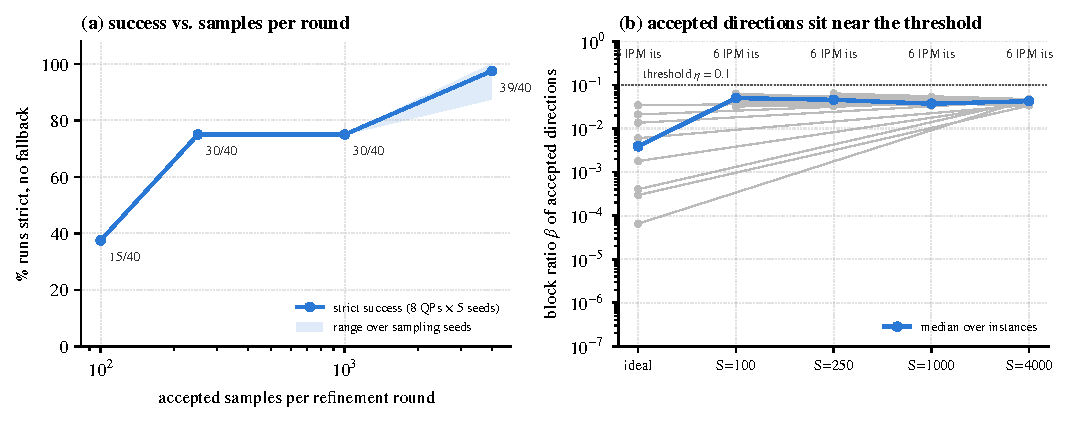
\includegraphics[width=\textwidth]{fig_shots.pdf}
\caption{Finite-shot polynomial solver over sampling seeds (session M). (a) Strict success versus accepted samples per refinement round; band: range over the five seeds. (b) Block ratio $\beta$ of the accepted directions per instance (grey) and median (blue), with the median number of IPM iterations above each group; dotted: the forcing threshold $\eta=0.1$.}\label{fig:shots}
\end{figure}

\subsection{The null-space target system}\label{sec:oss}
The null-space system~\eqref{eq:oss} is positive definite, so the polynomial~\eqref{eq:spdpoly} needs about $\sqrt\kappa$ rather than $\kappa$ walk steps. Table~\ref{tab:oss} and Fig.~\ref{fig:oss} compare both targets on the same 12 captured KKT systems, and the last two rows of Table~\ref{tab:integrated} run the null-space solver inside \texttt{coneqp}.

\lead{Early in the run the null space is cheaper; late in the run it is not.} At the first captured IPM iteration both targets have about the same condition number (median $19.9$ versus $19.4$), and the positive definite polynomial needs a median $12\times$ fewer walk steps ($2.5$--$834\times$). At the last captured iteration, the Jacobi-scaled null-space matrix has $\kappa_{\mathcal N}=4.2\times10^{5}$ (median) against $\kh=394$ for the equilibrated augmented matrix, because $Z\T SZ$ inherits the $\mu^{-2}$ growth of $S$, and it needs $1.6\times$ more walk steps---as Corollary~\ref{cor:oss} predicts, since $\sqrt{\kappa_{\mathcal N}}\approx650>2\kh$ only in the latter case. Over all 12 systems the median saving at $\eps=0.3$ is $3.0\times$, and the target is $2$--$4\times$ smaller ($n-p$ instead of $N$), which saves up to 11 qubits on the largest system.

\lead{With ideal readout the target works inside the IPM.} The null-space solver is strict and optimal on 8/8 instances, with a median of 40 walk steps per solve against 162 for the augmented solver on the same KKT matrices ($4.0\times$ fewer), 321 instead of 971 refinement rounds, and at most 23 qubits in both cases. Its post-selection probability, however, falls to $4.5\times10^{-13}$ (augmented: $3.8\times10^{-8}$), because $\norm{c}_1\approx\kappa_{\mathcal N}$.

\lead{With finite shots it fails.} At 250 samples per setting only 2/8 runs are strict: on five instances, the reference-branch reconstruction returns no usable estimate in one measurement setting, which yields a non-finite direction and stops the run, and on one instance the IPM uses a rejected direction. The completion~\eqref{eq:oss} explains the fragility: the multiplier $u_y$ is recovered through $P$, so that the readout error in $u_x$ is multiplied by $\norm{P}$. With ideal readout at $\eps=0.3$, the forward error of the completed direction is at most $0.14$ on the \ds{sanity} instances but $37$ on the first captured system of \ds{dense\_kappa\_n20\_k6\_s0} ($\kappa(P)=10^{6}$; Table~\ref{tab:oss}). Classically, CG on the null-space system needs $2.1\times$ fewer Krylov iterations than augmented MINRES on the dense families but not on the sparse ones (Fig.~\ref{fig:oss}c). The null-space target thus trades circuit depth for success probability and readout robustness: it is attractive early in the run and when $P$ is well conditioned, and a hybrid that switches to the augmented target as $\mu$ decreases is the natural next step.

\begin{table}[t]\centering\footnotesize
\caption{The same captured KKT systems as augmented (Ruiz-equilibrated, indefinite, odd optimal polynomial) and null-space (Jacobi-scaled, positive definite, shifted Chebyshev polynomial) targets at $\eps=0.3$ (session M). \emph{stage}: first, middle or last captured IPM iteration; $N$/dim: KKT and null-space dimension; $d$: walk steps; $p_{\text{succ}}$ and forward error of the completed direction for the null-space target with ideal readout.}\label{tab:oss}
\resizebox{\textwidth}{!}{%
\begin{tabular}{llrrrrrrrr}\toprule
instance & stage & $N$/dim & $\kh$ aug. & $\kappa_{\mathcal N}$ null & $d$ aug. & $d$ null & ratio & $p_{\text{succ}}$ null & fwd.\ err.\\\midrule
\inputrows{tex/oss_rows.tex}\bottomrule
\end{tabular}}
\end{table}

\begin{figure}[t]\centering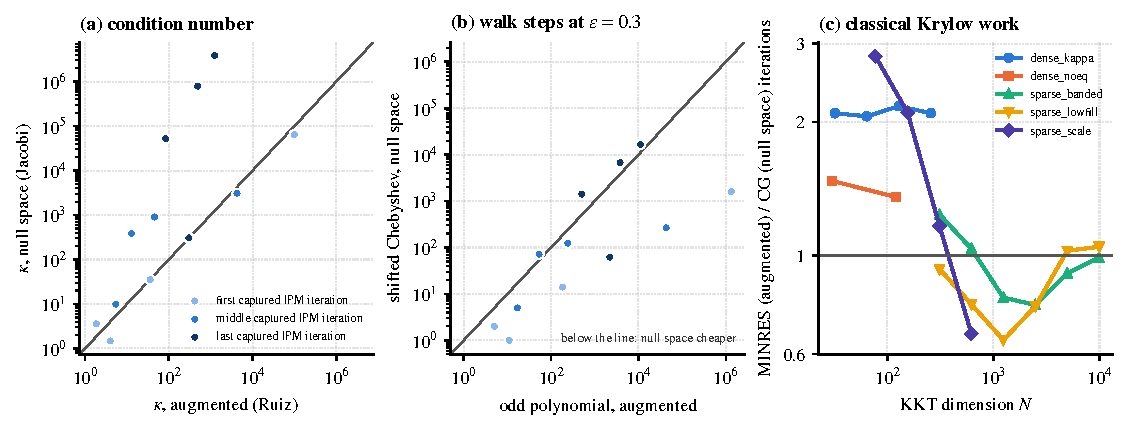
\includegraphics[width=\textwidth]{fig_oss.pdf}
\caption{Augmented versus null-space target (session M). (a) Condition numbers and (b) walk steps at $\eps=0.3$ on 12 captured systems, shaded by IPM progress; below the diagonal the null-space target is cheaper. (c) Classical Krylov work, MINRES on the augmented system over CG on the null-space system, per family and size.}\label{fig:oss}
\end{figure}

\subsection{Synthesis: quantum resource reductions and validation of the analysis}\label{sec:qresources}
Table~\ref{tab:resources} collects the resource reductions attributable to each methodological component, together with the theoretical prediction of Section~\ref{sec:theory}; Table~\ref{tab:equil} and Fig.~\ref{fig:qresources} provide the supporting measurements. All reductions are relative to alternative quantum configurations in the same simulation, not to classical solvers.

\lead{Equilibration.} Across all families, Ruiz equilibration lowers the maximum condition number along the IPM run by a median of $5.4\times10^{3}$ on \ds{dense\_kappa}, $4.3\times10^{4}$ on \ds{sparse\_banded}, $3.3\times10^{4}$ on \ds{sparse\_lowfill} and $7.5\times10^{4}$ on \ds{sparse\_scale} (Table~\ref{tab:equil}, Fig.~\ref{fig:qresources}a). By Corollary~\ref{cor:equil}, the corresponding degree of the optimal polynomial at $\eps=0.3$ falls by a median of $1.2\times10^{4}$ to $2.2\times10^{5}$; on the unscaled matrices, the median degree would exceed the simulation cap of $4\times10^{5}$ walk steps by factors of about 50 (\ds{dense\_kappa}) to 400 (\ds{sparse\_lowfill}), and it exceeds the cap on every instance of the three sparse families and on 85\,\% of the \ds{dense\_kappa} instances. On well-scaled matrices (\ds{sanity}, \ds{dense\_noeq}), the reduction is small (median $1.9$--$2.2$), and on some SDPLIB instances equilibration slightly increases $\kappa$ (minimum ratio $0.36$); the Maros--M\'esz\'aros matrices remain ill-conditioned after equilibration ($\kappa$ up to $4.2\times10^{15}$), so neither the classical nor the quantum solvers benefit there.

\lead{Readout model.} Fig.~\ref{fig:qresources}(b) confirms the empirical readout model of Remark~\ref{rem:readout}: with an accurate circuit, the contraction per round follows $\xi=c_0\sqrt{N/(2S)}$ with $c_0=\cZero$ over two orders of magnitude, independently of the polynomial and of $\kh$, and with $\eps=0.3$ it saturates at the polynomial error. The worst-case factor $\kh$ in~\eqref{eq:contraction} is not observed.

\lead{Classical work per solve.} Fig.~\ref{fig:qresources}(c) compares the classical matrix--vector products per KKT solve: 10--19 refinement rounds for the refined LCU solver at $N\le32$, against 24--27 MINRES iterations at the same sizes and up to $2\,061$ at $N=79\,360$. Under the empirical readout model with $S\propto N$, Theorem~\ref{thm:refine} predicts a number of rounds independent of $N$ (shaded band), whereas the MINRES count grows with $N$. The ratio $k/R$, which bounds any advantage by Proposition~\ref{prop:cost}, is at most $2.5$ at the simulated sizes.

\begin{table}[t]\centering\small
\caption{Effect of per-iteration Ruiz equilibration on the KKT condition number: per instance the maximum along the IPM run, then the median over the instances of a family (session M; sparse families for $N\le620$, where $\kappa$ was computed; SDPLIB: session A; Maros--M\'esz\'aros: offline diagnostic). \emph{degree red.}: median reduction of the optimal-polynomial degree at $\eps=0.3$ by~\eqref{eq:optdeg} (Corollary~\ref{cor:equil}).}\label{tab:equil}
\resizebox{\textwidth}{!}{%
\begin{tabular}{lrrrrrrr}\toprule
family & inst. & $N$ & $\kappa(\Kt)$ & $\kappa(D\Kt D)$ & reduction & range & degree red.\\\midrule
\inputrows{tex/equil_rows.tex}\bottomrule
\end{tabular}}
\end{table}

\begin{table}[t]\centering\small
\caption{Quantum resource reductions attributable to each methodological component (simulation; relative to alternative quantum configurations, not to classical solvers).}\label{tab:resources}
\begin{tabularx}{\textwidth}{p{3.3cm}p{2.1cm}p{3.0cm}Xp{1.5cm}}\toprule
component & resource & theory & measured reduction & source\\\midrule
\inputrows{tex/resources_rows.tex}\bottomrule
\end{tabularx}
\end{table}

\begin{figure}[t]\centering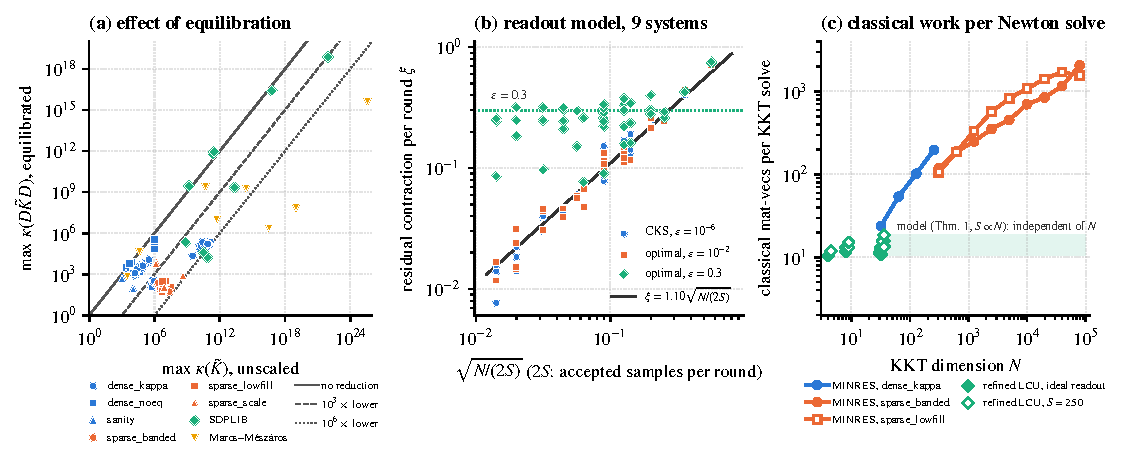
\includegraphics[width=\textwidth]{fig_qresources.pdf}
\caption{Quantum resource reductions. (a) Maximum condition number along the IPM run before and after Ruiz equilibration, per instance and family; lines mark no, $10^{3}\times$ and $10^{6}\times$ reduction. (b) Residual contraction per refinement round versus $\sqrt{N/(2S)}$ on 9 captured systems for three circuit settings, with the fitted readout model $\xi=c_0\sqrt{N/(2S)}$ (Remark~\ref{rem:readout}). (c) Classical matrix--vector products per KKT solve: MINRES iterations on three families against refinement rounds of the LCU solver with ideal and finite-shot readout; the band is the prediction of Theorem~\ref{thm:refine} with $S\propto N$.}\label{fig:qresources}
\end{figure}

\subsection{Comparison with published numerical studies}\label{sec:lit}
Table~\ref{tab:lit} places these results next to the numerical demonstrations we are aware of. Values in the rows marked $\dagger$ are taken from the cited papers and were not reproduced by us.

\begin{table}[t]\centering\small
\caption{Numerical studies of quantum linear solvers for optimisation. Values marked $\dagger$ are reported by the cited authors.}\label{tab:lit}
\begin{tabularx}{\textwidth}{p{3.5cm}XX}\toprule
study & setting & result\\\midrule
Mohammadisiahroudi et al.~\cite{mohammadisiahroudi2025improvements}$^\dagger$ & quantum IPM for LP; Qiskit HHL simulator; linear systems of dimension $\le16$ & inner and outer iterative refinement improve the precision from $\approx10^{-1}$ to $\approx10^{-4}$\\
Harkness et al.~\cite{harkness2026ir}$^\dagger$ & standalone linear systems; HHL with 3--5 clock qubits; dimension 8, $\kappa=5$ (simulator and IBM Heron); dimension 64 with 100--1000 shots & residual $\le10^{-9}$ in 9--10 rounds noiseless; $0.86\to0.07$--$0.10$ on hardware; $10^{-3}$ in $\approx10$ rounds with 100 shots\\
Dalzell et al.~\cite{dalzell2023endtoend}$^\dagger$ & resource estimate (no simulation) of a quantum IPM for a 100-asset portfolio SOCP & $\approx8\times10^{6}$ logical qubits and $\approx7\times10^{29}$ T gates; tomography and $\kappa$ dominate\\
Ozbaygin et al.~\cite{ozbaygin2026vqe}$^\dagger$ & VQE as separation oracle in an SDP cutting-plane scheme; SDPLIB \ds{control1}--\ds{control10}; simulator, noise model, IBM hardware & valid cuts throughout; 32--82\,\% of the initial gap closed versus 75--82\,\% with exact eigendecomposition; oracle $10^{3}$--$10^{4}\times$ slower; matrices $\ge98\,\%$ dense in the Pauli basis\\
this work & convex QP inside unmodified \textsc{cvxopt}; LCU polynomial solver at the walk level with low-precision refinement; KKT dimension $\le32$ inside the IPM, $\kappa\le3.8\times10^{4}$; strict no-fallback accounting; six sessions & 8/8 strict with ideal readout; 38--98\,\% with 100--$4\,000$ samples per round over 5 seeds; $237\times$ fewer queries than a high-precision circuit; $8.2\times10^{12}$ queries at 500 samples per round; HHL 2/4; null-space target $4.0\times$ shallower, 2/8 with finite shots\\\bottomrule
\end{tabularx}
\end{table}

\section{Discussion}\label{sec:discussion}
\subsection{Significance of the methodological contributions}
The study examined, inside an unmodified production IPM and under one acceptance test, one fallback protocol and one accounting, what accuracy a Newton direction must have, how it can be certified, and which classical and quantum solvers deliver it. Five findings are of general significance.

\lead{Equilibration, not the acceptance test, makes an unpreconditioned Krylov solver reliable on regular problems.} Every Ruiz-equilibrated variant with a tolerance of $10^{-10}$ or tighter is fallback-free on 100\,\% of the synthetic runs, whereas every unscaled variant needs fallback in 38--50\,\% of them. The equilibrated augmented matrix has $\kappa\in[80,180]$ along a run in which the NT scaling spreads over six orders of magnitude---the measured form of the boundedness theory for unreduced KKT systems. On the Maros--M\'esz\'aros QPs, which violate the assumptions of that theory, the same matrix reaches $\kappa=4.2\times10^{15}$ and MINRES needs fallback on more than half of the instances.

\lead{Fill-in and regularity, not the method, decide whether the iterative solver is faster.} Under high fill-in the crossover is at $N\approx5\times10^{3}$ and the advantage reaches $9.4\times$ at $N\approx2\times10^{4}$, with less than $\pm30\,\%$ spread over instances; under low fill-in there is no crossover below $N\approx4\times10^{4}$; and on 48 real-world QPs the solver's own factorisation is fastest on 40. Latency, not arithmetic, sets the useful range of a GPU Krylov kernel: the mat-vec is $13.4\times$ faster on the T4 at $N=79\,360$, but a baseline MINRES iteration costs a constant $0.7$\,ms; one synchronisation per iteration and fused updates recover $1.14$--$1.29\times$, and the GPU pays off from $N\approx2\times10^{4}$.

\lead{A Newton direction needs a relative forward error between $\tau/10$ and $\tau$.} This precision law, measured at every tolerance from $10^{-8}$ to $10^{-4}$, is the accuracy target for any inexact solver. A backward-error certificate alone is insufficient when $\kappa(\Kt)$ is large (Lemma~\ref{lem:fwd}); the per-block forcing test supplies the IPM-specific structure and binds on the equality block late in the run, which is where the 22--34\,\% over-solving of the combined test originates and what an IPM-aware stopping rule~\cite{zanetti2023stopping} could recover.

\lead{Low-precision refinement is the decisive design choice for a quantum KKT solver.} Inside the linear solve, refinement converges for any solver with $\xi<1$, which the polynomial solver guarantees by construction and HHL achieves only where its clock resolves the spectrum. Operating the circuit at $\eps=0.3$ with a few hundred samples per round is $237$--$624\times$ cheaper in queries than a high-precision circuit, keeps the circuit depth independent of the IPM tolerance (Corollary~\ref{cor:precision}), and replaces the $\bigO(N/\tau^2)$ samples of direct readout by $\bigO(N\log(1/\tau))$---\directSamples{} versus \refinedSamples{} samples per solve at the default tolerance.

\lead{The forcing threshold interacts with the cost of a quantum solver.} With finite shots, refinement stops at directions whose block ratio is close to $\eta$; such directions add IPM iterations, and the additional iterations reach barrier parameters at which the KKT matrix, and hence the circuit depth, grows by an order of magnitude. A quantum solver inside an IPM should therefore be run with a tighter forcing parameter than a classical one, and its cost model must include the effect of $\eta$ on the number of IPM iterations.

\subsection{Outlook for a quantum advantage}
The results do not demonstrate a quantum advantage, and the analysis explains why none is possible at the simulated sizes: for $N\le32$ the ratio $k/R$ is at most $2.5$, and the query counts exceed the classical cost by many orders of magnitude. The analysis also identifies the regime in which the methodology could yield one. Proposition~\ref{prop:cost} requires dense, well-equilibrated KKT systems---large $\bar\nu$ and moderate $\kh$---solved to IPM accuracy by low-precision refined circuits with $S=\Theta(N)$ samples, on hardware whose block-encoding queries do not grow with $\nnz(\Kt)$, and preferably with an optimal-scaling QLSA ($\gamma=1$). In that regime the advantage is polynomial, bounded by $k/R$, and grows with the classical iteration count, which on \ds{dense\_kappa} increases from 24 to 198 between $N=32$ and $N=256$ while $R$ does not. Each methodological component moves the cost towards this regime: equilibration lowers $\kh$, which enters as $\kh^{\gamma}$, by three to five orders of magnitude; low-precision refinement removes the $1/\eps_f^2$ sample dependence and fixes the depth; the optimal polynomial reduces the queries per accepted sample by $4.8\times$; and the null-space target reduces the depth by the factor $2\kh/\sqrt{\kappa_{\mathcal N}}$ where Corollary~\ref{cor:oss} applies. Because these components are classical pre- and post-processing steps, they apply unchanged to other QLSA-based IPMs and to optimal-scaling solvers~\cite{costa2022optimal,dalzell2024shortcut}, which would remove the post-selection factor $\norm{c}_1$; the coherent tomography of~\cite{vanapeldoorn2023tomography} would improve the sample dependence further. As in the VQE cutting-plane study~\cite{ozbaygin2026vqe}, the readout of a classical vector, not the preparation of the solution state, remains the dominant obstacle that a hardware realisation would have to overcome.

\subsection{Limitations}
The quantum results are classical simulations of ideal circuits that assume free block encoding, state preparation, knowledge of $\kappa$ and ideal amplitude amplification; the KKT systems inside the IPM have dimension at most 32, and success counts beyond $\kappa\approx4\times10^{4}$ are limited by the simulation's depth cap rather than by the algorithm. The empirical readout model is fitted on systems with $N\le64$, and the instantiation of Proposition~\ref{prop:cost} at larger $N$ is an extrapolation under stated assumptions. The Maros--M\'esz\'aros subset stops at $N\approx10^{4}$ and excludes instances on which \texttt{coneqp} itself fails; the condition-number diagnostic covers eight of its instances. The claims do not extend to SDP (Appendix~\ref{app:sdplib}), and we have not compared against GPU direct solvers~\cite{chen2025cuclarabel} or first-order GPU solvers~\cite{lu2025cupdlp}. The largest synthetic sizes rest on two instances (\ds{sparse\_banded}) or one (\ds{sparse\_lowfill}), replicated in further sessions. Timings vary by up to $1.3\times$ in the median between CPU-only and GPU sessions.

\subsection{Directions for future research}
On the classical side, the real-world results call for a preconditioner or regularisation that restores bounded conditioning on degenerate problems---primal--dual regularisation as in interior-point proximal methods~\cite{pougkakiotis2021ippmm} combined with general-purpose preconditioners~\cite{gondzio2022generalpurpose,bergamaschi2004preconditioning} is the natural candidate, and the exact-deflation bound of Section~\ref{sec:spectrum} ($3.7$--$6.2\times$) is the gap that a better source of approximate eigenvectors than Lanczos harvesting~\cite{luo2024neurkitt} would have to close. On the quantum side, the forcing parameter should be chosen jointly with the sample count; a hybrid target---null space early in the run, augmented late, switched by the criterion of Corollary~\ref{cor:oss}---would combine the $\sqrt{\kappa}$ degree of the first with the robustness of the second; and testing the readout model and the conditions of Proposition~\ref{prop:cost} on larger dense systems, with resource estimates for concrete block encodings, would determine whether the advantage regime identified here is reachable.

\section{Conclusion}\label{sec:conclusion}
We have presented a certified framework for replacing the KKT factorisation of a production interior-point solver by classical Krylov or simulated quantum linear solvers, and four methodological components that make such replacements reliable and economical: per-iteration symmetric equilibration, a combined block-forcing and backward-error acceptance test, a latency-optimised GPU MINRES kernel, and a low-precision refined polynomial quantum solver with an optional positive definite null-space target. On the classical side, equilibrated MINRES is fallback-free on all synthetic runs, up to $9.4\times$ faster than sparse LDL$\T$ under high fill-in and $3.75\times$ faster on the GPU at $N=79\,360$, while low fill-in and degenerate real-world QPs mark the limits of these gains. A Newton direction needs a relative error between $\tau/10$ and $\tau$. On the quantum side, we proved contraction, round and query bounds for the refined solver and derived how precision, equilibration and the choice of target enter them; in simulation, these components reduce the block-encoding queries per solve by $237\times$, the circuit depth by $2.70\times$ and a further $4.0\times$, and the samples per solve by more than thirteen orders of magnitude relative to direct readout, and the IPM converges on quantum-produced directions alone on 8/8 instances with ideal readout and on 39/40 seeded runs with finite sampling. Proposition~\ref{prop:cost} shows that these reductions could translate into a polynomial advantage over classical MINRES only for dense, well-equilibrated systems at sizes far beyond those simulated, and only on hardware with inexpensive block encodings. All quantum results are classical simulations of ideal circuits; no end-to-end quantum speed-up is demonstrated or claimed.

\appendix
\section{Reproducibility}\label{app:repro}
All results are produced by a single Jupyter notebook in two builds (CPU and GPU), which runs on Kaggle with the problem-size profile selected in its configuration cell (\texttt{smoke}, \texttt{small}, \texttt{medium} or \texttt{large}). The notebook installs Qiskit for the cross-check, downloads the Maros--M\'esz\'aros files when Internet access is enabled, records software versions, hardware and seeds in \path{environment.json} and \path{config.json} (with a configuration hash), and writes every table of this paper as CSV---among them \path{benchmark_results.csv}, \path{linear_solve_logs.csv}, \path{quantum_results.csv}, \path{qls_comparison_hhl_vs_cks.csv}, \path{oss_target_comparison.csv}, \path{performance_profiles.csv}, \path{maros_meszaros_instances.csv}, \path{outer_refinement.csv}, \path{gpu_matvec_benchmark.csv}, \path{failures.csv} and \path{experiment_status.csv}; peak memory is a column of \path{benchmark_results.csv}---together with the captured KKT systems and an automatically generated report, and compresses them into one result bundle per session. The tables of this paper are extracted from the bundles by \path{extract_tables_main.py} (sessions M and B--E) and \path{extract_tables_sessionA.py} (session A); the LaTeX bodies of the result tables are generated from the extracted CSV files by \path{make_tex_tables.py}, so that no measured number in them is copied by hand (Table~\ref{tab:notadopted} is a typed summary that also draws on exploratory runs on the same instances), and the figures are generated by \path{make_figures.py}. The condition-number diagnostic of Fig.~\ref{fig:realqp}(b) is computed by \path{mm_kappa_diag.py}, which runs the notebook's own solver code on eight Maros--M\'esz\'aros instances. Random seeds are derived from a global seed (20260911) and the instance and method names, so that every instance and every quantum sample is reproducible.

\section{SDPLIB}\label{app:sdplib}
Ten SDPLIB instances were solved with \texttt{conelp} under the same protocol (Table~\ref{tab:sdplib}, session A). In this session the inexact methods were run on instances with $N\le350$, i.e.\ on the seven instances \ds{truss1}, \ds{truss4}, \ds{hinf1}, \ds{hinf2}, \ds{control1}, \ds{truss3} and \ds{control2}; \ds{truss2}, \ds{qap5} and \ds{theta1} were solved only by the direct solvers, and \ds{theta1} exceeds the size limit of the reference LU decomposition. The combined test is accepted on 4 of the 7 instances, with $1\,048$ fallbacks in total; the tightest backward-error test ($10^{-12}$) on 6 of 7, with 361 fallbacks; and the block test alone on none, with $1\,483$ fallbacks. The equilibrated KKT matrices reach condition numbers of $2.7\times10^{9}$ (\ds{control1}) to $1.8\times10^{19}$ (\ds{hinf1}). The claims of this paper are therefore restricted to QP.

\begin{table}[h]\centering\small
\caption{SDPLIB per instance (\texttt{conelp}, session A). \emph{its}: IPM iterations of the unmodified solver; \emph{acc.}: final tolerance reached (fallback allowed); \emph{fb}: total classical fallbacks of the MINRES variant; $\kappa(D\Kt D)$: largest equilibrated condition number along the exact-LU run. ``--'': not run.}\label{tab:sdplib}
\resizebox{\textwidth}{!}{%
\begin{tabular}{lrr|r|rr|rr|r|r}\toprule
 & & & LDL$\T$ & \multicolumn{2}{c|}{MINRES, combined} & \multicolumn{2}{c|}{MINRES, backward $10^{-12}$} & block $\eta=0.1$ & \\
instance & $N$ & its & acc. & acc. & fb & acc. & fb & fb & $\kappa(D\Kt D)$\\\midrule
\inputrows{tex/sdplib_rows.tex}\bottomrule
\end{tabular}}
\end{table}

\section{Replication across sessions}\label{app:replication}
Sessions B (GPU, medium profile, 21 September 2026), C (GPU, small profile, 24 September), D (CPU, small profile, 26 September) and E (CPU, medium profile, 27 September) were executed on different Kaggle machines from the main session M. All six sessions use the same instance generator and seeds, so the synthetic instances they share are identical (session B: seeds 0 and 1; sessions C and D: seed 0; session D runs the CPU methods up to $N=9\,920$; session E runs the complete experiment set of M with the GPU methods omitted). In every session, all classical methods were accepted and strict on the synthetic sparse families with zero fallbacks and with the IPM iteration counts of session M (in session E on all 550 runs).

Table~\ref{tab:replication} gives, per method and family, the median and the 10--90\,\% range over (instance, size) pairs of the ratio of a session's whole-run time to that of session M. The two GPU sessions agree with M to within $0.96$--$1.10$ in the median. The CPU-only sessions run the direct solvers $6$--$31\,\%$ slower, and session E also runs MINRES $12$--$16\,\%$ slower, which is why all speed-ups in the paper are computed within one session. Table~\ref{tab:crossovers} lists the quantities on which the conclusions rest for every session, and Fig.~\ref{fig:replication} plots the per-size ratios.

\begin{table}[h]\centering\small
\caption{Whole-run wall time of a replication session divided by that of session M, per method: median (10--90\,\% range) over the instances and sizes both sessions ran.}\label{tab:replication}
\resizebox{\textwidth}{!}{%
\begin{tabular}{lrrrr}\toprule
method & B: GPU, medium & C: GPU, small & D: CPU, small & E: CPU, medium\\\midrule
\inputrows{tex/replication_rows.tex}\bottomrule
\end{tabular}}
\end{table}

\begin{table}[h]\centering\small
\caption{Crossover quantities, quantum success counts and further replicated quantities in each session (speed-ups are medians of per-instance paired ratios within the session; ``--'': not run in that session; session D runs 7 of the 8 quantum instances and 13 Maros--M\'esz\'aros instances).}\label{tab:crossovers}
\resizebox{\textwidth}{!}{%
\begin{tabular}{lrrrrr}\toprule
quantity & M & B & C & D & E\\\midrule
\inputrows{tex/crossover_rows.tex}\bottomrule
\end{tabular}}
\end{table}

\begin{figure}[h]\centering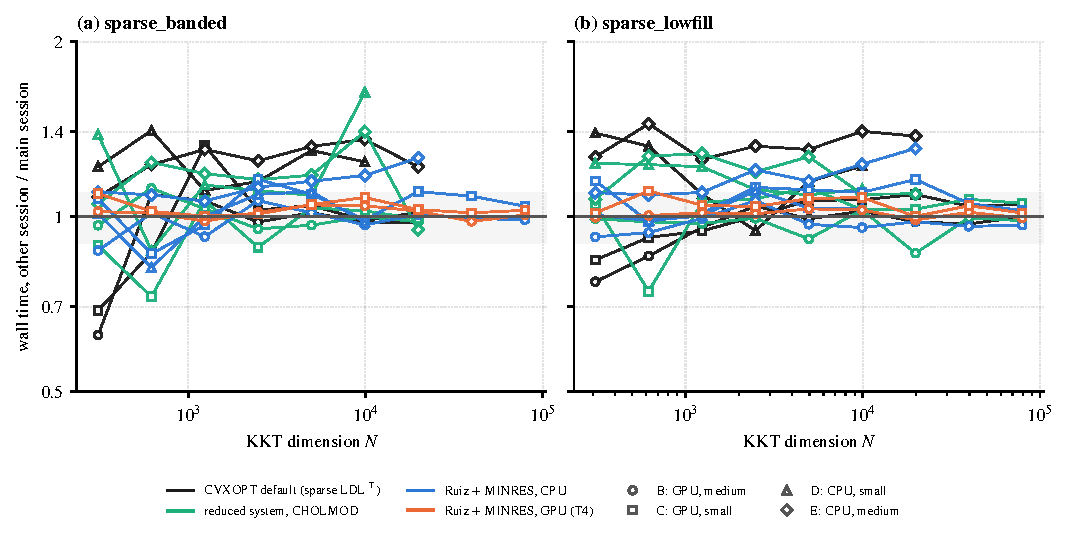
\includegraphics[width=\textwidth]{fig_replication.pdf}
\caption{Ratio of the whole-run wall time in sessions B--E to that in session M, per method and size; the band marks $\pm10\,\%$.}\label{fig:replication}
\end{figure}

\clearpage
\bibliographystyle{plainnat}
\bibliography{refs}
\end{document}
